\documentclass[11pt]{article}
    \title{\textbf{Sistema prenotazione lezioni}}
    \author{Vincenzo Imperati 1834930}
    \date{}
    \usepackage{graphicx}
    \usepackage[dvipsnames]{xcolor}
	\usepackage{tabularx,booktabs}
	\usepackage{float}
	\usepackage{tabto}    
	\usepackage{hyperref}

\begin{document}

\maketitle
\thispagestyle{empty}


\begin{abstract}
Progettare un sistema di prenotazione di posto a lezione, nel rispetto della (nuova) capienza delle aule (caratterizzate da un codice).
\\\indent
La presenza degli studenti è organizzata in turni prenotabili in base alle ultime due cifre del numero di matricola (da 00 a 49 e da 50 a 99) a settimane alterne.
\\\indent
La prenotazione per ciascun turno può essere fatta (e cancellata,per permettere a studenti in lista d’attesa di frequentare) solo dal lunedì a venerdì della settimana precedente.
\\\indent
Al termine della prenotazione, il sistema produce una ricevuta (con aula, matricola ed orario) da scaricare/salvare.
\\\indent
Per accedere al sistema servono le credenziali di Sapienza.
\end{abstract}

\newpage
\tableofcontents
\newpage

\section{Analisi di contesto}
Si vuole progettare un portale web per permettere agli studenti dell'Università degli Studi di Roma "La Sapienza" di prenotare il proprio posto in aula, nel rispetto della nuova capienza della aule.
Il sistema dovrá necessariamente:
\begin{itemize}
\itemsep0em
\item permettere agli utenti di effettuare il login tramite le proprie credenziali del sistema Infostud;
\item permettere agli studenti di effettuare e gestire prenotazioni;
\item permettere ai docenti di creare e gestire eventi;
\end{itemize}
Il sistema si appoggia ad alcune funzionalitá del sistema esterno Infostud:
\begin{itemize}
\itemsep0em
\item Accesso
\item Logout
\end{itemize}

\subsection{Glossario}
Di seguito vengono descritte alcune terminologie:
\begin{description}
\addtolength{\itemindent}{0.5cm}
\itemsep0em
\item [Evento] Entità di cui è possibile effettuare la prenotazione, ad esempio: "Lezione di ingegneria del software in aula Cabibbo il giorno 01-01-2021 dalle 8:00 alle 11:00 tenuta dal professor Parisi-Presicce" (lo studente prenoterà un evento, equivalente a dire: lo studente prenoterà un posto in una determinata aula in un determinato giorno per un determinato intervallo di tempo). L'evento è quindi composto da nome evento (nome descrittivo dell'evento), aula (della quale si vuole occupare un posto e nella quale l'evento si svolge), data e intervallo di tempo (il periodo di tempo del giorno in cui l'evento si svolge), intestatario (il soggetto che ha creato l'evento).
\item [Prenotazione valida] Prenotazione effettuata andata a buon fine. Questo tipo di prenotazione rispetta i vincoli imposti dal sistema riguardanti la validità delle prenotazioni. Questo tipo di evento è prenotabile dagli studenti.
\item [Prenotazione cancellata] Prenotazione non piú valida o non piú in attesa. Questo tipo di prenotazione era precedentemente: una prenotazione valida, poi cancellata dallo studente intestatario; oppure una prenotazione in attesa che non ha ottenuto esito positivo (non si è tramutata in prenotazione valida).
\item [Prenotazione in attesa] Prenotazione effettuata con possibilità di essere validata o cancellata. Questa prenotazione è nella lista delle prenotazioni in attesa di un determinato evento. Diventa valida quando si libera un posto per quel determinato evento e si esce dalla lista di attesa perché si ha la precedenza rispetto alle altre prenotazioni in attesa della stessa lista di ettesa. Diventa cancellata quando scade il termine di prenotazione dell'evento in cui la prenotazione è ancora in lista di attesa, oppure quando viene cancellato l'evento.
\item [Prenotazione scaduta] Prenotazione non piú valida una volta che l'evento a cui la prenotazione fa riferimento è terminato.
\item [Evento valido] Evento creato andato a buon fine. Questo tipo di evento rispetta i vincoli imposti dal sistema riguardanti la validità della creazione di eventi.
\item [Evento cancellato] Evento non piú valido o non piú in attesa. Questo tipo di evento era precedentemente: un evento valido, poi cancellato dal docente intestatario; oppure un evento in attesa che non ha ottenuto esito positivo (la segreteria amministrativa non ha validato l'evento).
\item [Evento in attesa] Evento creato con possibilità di essere validato o cancellato. Questo evento è nella lista generale degli eventi in attesa. Diventa valido quando la segreteria amministrativa valida l'evento. Diventa cancellato quando la segreteria per qualche motivo in valida l'evento.
\item [Evento terminato] Evento non piú valido una volta che l'evento è terminato.
\item [Lista generale degli eventi di ettesa] Lista univoca di tutti gli eventi creati dai docenti in attesa di essere validati dalla segreteria amministrativa;
\item [Lista di attesa di un evento] Lista delle prenotazioni effettuate dagli studenti per un dato evento in attesa di essere validate dal sistema di validazione automatico. In questa lista restano in attesa le prenotazioni effettuate dopo il superamento dei posti totali disponibili dell'aula che ospita il dato evento;
\item [Matricola e settimana concorde] Definizione per cui la matricola in questione rispetta i vincoli di prenotazione del sistema rispetto alla settimana in questione. Ovvero è possibile per quella matricola prenotare eventi per quella settimana siccome rispetta i vincoli di prenotazione del sistema.
\item [Matricola e settimana discorde] Definizione per cui la matricola in questione non rispetta i vincoli di prenotazione del sistema rispetto alla settimana in questione. Ovvero non è possibile per quella matricola prenotare eventi per quella settimana siccome non rispetta i vincoli di prenotazione del sistema.
\end{description}
\newpage

\section{Specifica dei requisiti}

\subsection{Requisiti funzionali}
Il sistema dovrà permettere allo studente iscritto alla Sapienza di svolgere nel portale web le seguenti attività:
\begin{description}
\addtolength{\itemindent}{0.5cm}
\itemsep0em
\item [RF\_STUDENTE\_01\_Accesso] Accedere al portale web attraverso le proprie credenziali Sapienza;
\item [RF\_STUDENTE\_02\_Logout] Effettuare il logout dal portale web;
\item [RF\_STUDENTE\_03\_Effettua-prenotazioni] Effetuare la prenotazione di eventi rispettando V\_STUDENTE\_01\_Un-solo-posto, V\_STUDENTE\_02\_Settimana-matricola-concorde e V\_STUDENTE\_03\_Finestra-prenotazioni;
\item [RF\_STUDENTE\_04\_Cancella-prenotazioni] Cancellare la prenotazione di eventi rispettando V\_STUDENTE\_03\_Finestra-prenotazioni e V\_STUDENTE\_04\_Cancellazione-prenotazioni;
\item [RF\_STUDENTE\_05\_Visualizza-prenotazioni-effettuate] Visualizzare le prenotazioni effettuate;
\item [RF\_STUDENTE\_06\_Scarica-ricevute-prenotazioni] Scaricare le ricevute delle prenotazioni valide effettuate;
\item [RF\_STUDENTE\_07\_Visualizza-lista-attesa] Visualizzare la lista di attesa dell'evento prenotato in caso di prenotazione in attesa;
\item [RF\_STUDENTE\_08\_Ricerca-aule] Ricercare le aule tramite il loro codice identificativo;
\item [RF\_STUDENTE\_09\_Ricerca-eventi] Ricercare gli eventi tramite il loro codice identificativo;
\item [RF\_STUDENTE\_10\_Visualizza-info-aule] Visualizzare le informazioni delle aule;
\item [RF\_STUDENTE\_11\_Visualizza-info-eventi] Visualizzare le informazioni degli eventi.
\end{description}
Il sistema dovrà permettere al docente iscritto alla Sapienza di svolgere nel portale web tutte le seguenti attività:
\begin{description}
\addtolength{\itemindent}{0.5cm}
\itemsep0em
\item [RF\_DOCENTE\_01\_Accesso] Accedere al portale web attraverso le proprie credenziali Sapienza;
\item [RF\_DOCENTE\_02\_Logout] Effettuare il logout dal portale web;
\item [RF\_DOCENTE\_03\_Crea-eventi] Creare un evento rispettando V\_DOCENTE\_01\_Creazione-eventi;
\item [RF\_DOCENTE\_04\_Cancella-eventi] Cancellare un evento rispettando V\_DOCENTE\_02\_Cancellazione-eventi;
\item [RF\_DOCENTE\_05\_Visualizza-eventi-creati] Visualizzare gli eventi creati;
\item [RF\_DOCENTE\_06\_Scarica-ricevute-eventi] Scaricare le ricevute degli eventi validi creati;
\item [RF\_DOCENTE\_07\_Visualizza-lista-generale-attesa] Visualizzare la lista generale degli eventi in attesa;
\item [RF\_DOCENTE\_08\_Ricerca-aule] Ricercare le aule tramite il loro codice identificativo;
\item [RF\_DOCENTE\_09\_Ricerca-eventi] Ricercare gli eventi tramite il loro codice identificativo;
\item [RF\_DOCENTE\_10\_Visualizza-info-aule] Visualizzare le informazioni delle aule;
\item [RF\_DOCENTE\_11\_Visualizza-info-eventi] Visualizzare le informazioni degli eventi.
\end{description}
Il sistema dovrà permettere alla segreteria amministrativa di svolgere nel portale web tutte le seguenti attività:
\begin{description}
\addtolength{\itemindent}{0.5cm}
\itemsep0em
\item [RF\_SEGRETERIA\_01\_Accesso] Accedere al portale web attraverso le proprie credenziali Sapienza;
\item [RF\_SEGRETERIA\_02\_Logout] Effettuare il logout dal portale web;
\item [RF\_SEGRETERIA\_03\_Valida-eventi] Validare gli eventi in attesa;
\item [RF\_SEGRETERIA\_04\_Invalida-eventi] Invalidare gli eventi in attesa;
\item [RF\_SEGRETERIA\_05\_Visualizza-lista-generale-attesa] Visualizzare la lista generale degli eventi in attesa;
\item [RF\_SEGRETERIA\_06\_Ricerca-aule] Ricercare le aule tramite il loro codice identificativo;
\item [RF\_SEGRETERIA\_07\_Ricerca-eventi] Ricercare gli eventi tramite il loro codice identificativo;
\item [RF\_SEGRETERIA\_08\_Visualizza-info-aule] Visualizzare le informazioni delle aule;
\item [RF\_SEGRETERIA\_09\_Visualizza-info-eventi] Visualizzare le informazioni degli eventi.
\end{description}

\subsection{Requisiti non funzionali}
Il sistema dovrà soddisfare tutti i seguenti requisiti non funzionali:
\begin{description}
\addtolength{\itemindent}{0.5cm}
\itemsep0em
\item [RNF\_SISTEMA\_01\_Usabilità] Il sistema dovrà avere un'interfaccia intuitiva per permettere a tutti gli utenti di usare agevolmente il portale web;
\item [RNF\_SISTEMA\_02\_Disponibilità] Il sistema dovrà essere disponibile nel 99,99\% del tempo; 
\item [RNF\_SISTEMA\_03\_Affidabilità] Il sistema dovrà eseguire un backup del database ogni giorno;
\item [RNF\_SISTEMA\_04\_Prestazione] Il sistema dovrà garantire un tempo di risposta medio tra 1 e 4 secondi per svolgere le richieste dell'utente. Nel caso in cui ció non è possibile, dovrà essere mostrato all'utente un messaggio di attesa dell'operazione in corso. Nel caso in cui la richiesta supera i 15 secondi, essa dovrà essere annullata e dovrà essere mostrato all'utente un messaggio di operazione fallita;
\item [RNF\_SISTEMA\_05\_Sicurezza] Il sistema dovrà garantire la riservatezza dei dati sensibili degli utenti.
\end{description}

\subsection{Vincoli}
Il sistema dovrà rispettare tutti i seguenti vincoli:
\begin{description}
\addtolength{\itemindent}{0.5cm}
\itemsep0em
\item [V\_STUDENTE\_01\_Un-solo-posto] Lo studente potrà prenotare solo un posto per evento;
\item [V\_STUDENTE\_02\_Settimana-matricola-concorde]Lo studente potrà prenotare i posti in aula solo per le settimane consentitegli secondo il proprio numero di matricola;
\item [V\_STUDENTE\_03\_Finestra-prenotazioni] Lo studente potrà effettuare o cancellare una prenotazione dal lunedí al venerdí della settimana precedente a quella dell'effettiva prenotazione;
\item [V\_STUDENTE\_04\_Cancellazione-prenotazioni] Lo studente potrà cancellare solo prenotazioni valide o in attesa da lui precedentemente effettuate;
\item [V\_DOCENTE\_01\_Creazione-eventi] Il docente potrà creare solo eventi con data e intervallo non intersecabile con altri eventi validi già da lui creati;
\item [V\_DOCENTE\_02\_Cancellazione-eventi] Il docente potrà cancellare solo eventi validi o in attesa da lui precedentemente creati;
\item [V\_AULA\_01\_Capienza] Le prenotazioni valide per ogni evento non devono superare la nuova capienza dell'aula in cui l'evento ha luogo.
\end{description}

\newpage

\section{Analisi}

\subsection{Casi d'uso e analisi nomi/verbi}
Di seguito vengono descritti nel dettaglio i casi d'uso e ad essi viene fatta l'analisi nomi/verbi:
\begin{itemize}
\itemsep0em
\item In \colorbox{red}{rosso} sono evidenziati i nomi, potenziali candidati a divenire classi o attributi;
\item In \colorbox{green}{verde} sono evidenziati i verbi, potenziali candidati a divenire responsabilità di classe;
\item In \colorbox{cyan}{azzurro} sono evidenziati i predicati nominali, potenziali candidati per divenire attributi o in alcuni casi classi.
\end{itemize}

\begin{figure}[H]
\centering
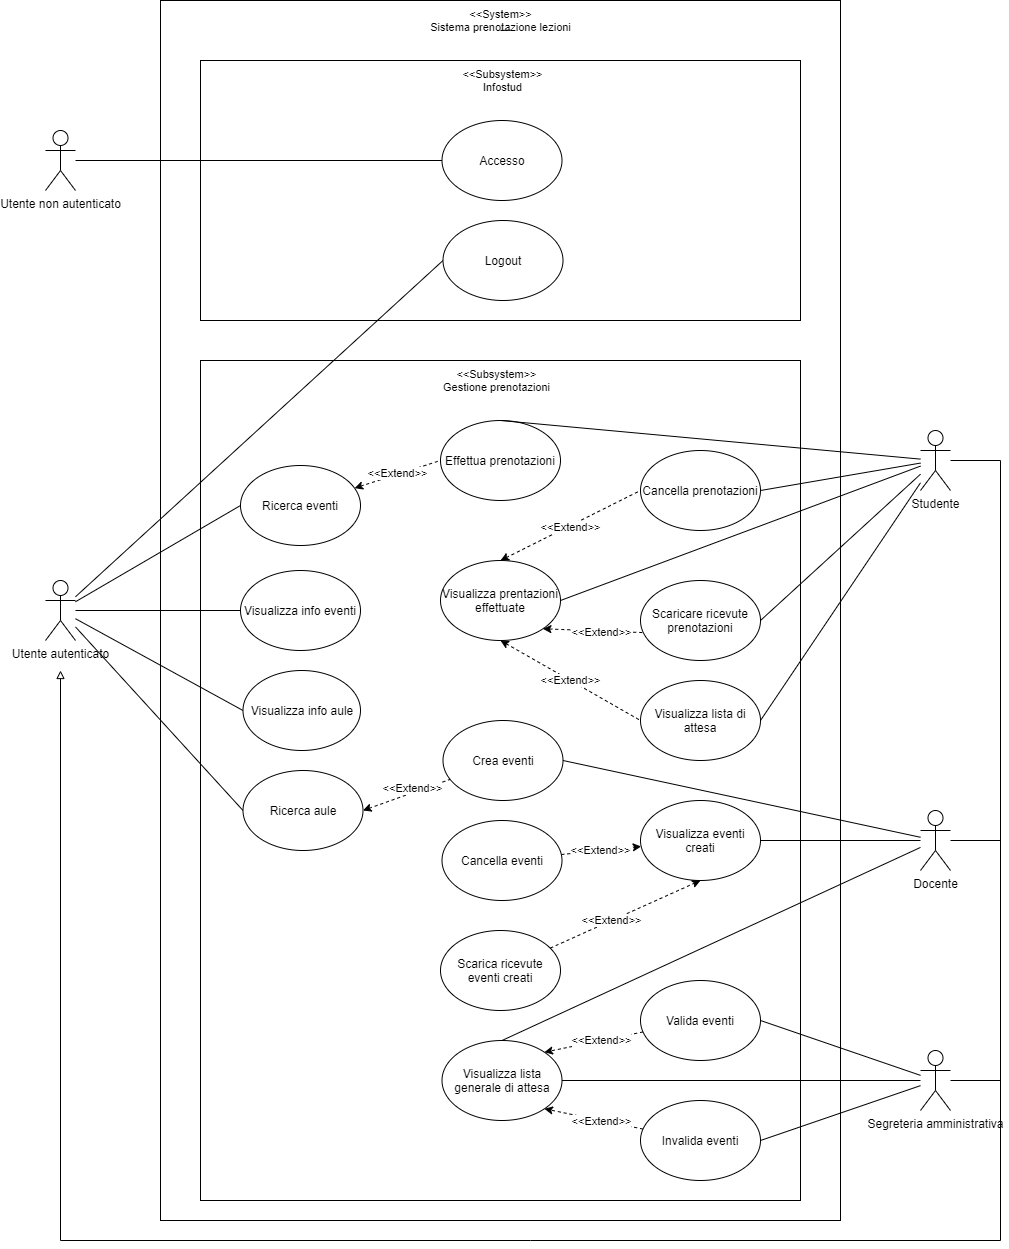
\includegraphics[width=1\textwidth]{Diagramma use-case.png}
\caption{Diagramma use-case}
\end{figure}

\begin{table}[H]
\centering
\begin{tabularx}{1\textwidth}{|l|X|}
\hline
\multicolumn{2}{|c|}{\textbf{UC\_01\_Accesso}}\\
\hline \textbf{Attori} & \colorbox{red}{Utente non autenticato} (di seguito utente)\\
\hline \textbf{Descrizione} & \colorbox{green}{Accedere} al portale web attraverso le proprie \colorbox{cyan}{credenziali Sapienza}\\
\hline \textbf{Pre-condizioni} & IL sistema non contiene una sessione attiva dell'utente\\
\hline \textbf{Flusso principale} &
1. L'\colorbox{red}{utente} \colorbox{green}{accede} ad una qualsiasi pagina del sito web;

2. Il sistema \colorbox{green}{chiede} all'\colorbox{red}{utente} di \colorbox{green}{inserire} le proprie \colorbox{cyan}{credenziali Sapienza} per l'\colorbox{green}{autenticazione};

3. L'\colorbox{red}{utente} \colorbox{green}{compila} e \colorbox{green}{conferma} i dati inseriti;

4. Infostud \colorbox{green}{trova} l'utente con quei dati associati è \colorbox{green}{comunica} l'avvenuta identificazione al sistema;

5. Il sistema \colorbox{green}{reindirizza} l'utente alla pagina principale in base al
suo ruolo all'interno del sistema (Studente, Docente,
Segreteria amministrativa).
\\
\hline \textbf{Post-condizioni} & Il sistema contiene una sessione attiva dell'utente\\
\hline \textbf{Flusso alternativo \#1} & 
4.a. Infostud comunica al sistema che non esiste un utente con quei dati associati;

4.a.1. Il sistema segnala l'errore all'utente e chiede di inserire nuovamente i dati;

4.a.2. Il flusso riprende dal punto 3. del flusso principale
\\
\hline \textbf{Flusso alternativo \#2} & 
4.b. Il Sistema rileva che non tutti i campi obbligatori sono stati compilati;

4.b.1. Il Sistema segnala l'errore all'utente e chiede di inserire nuovamente i;
dati;

4.b.2. Il flusso riprende dal punto 3. del flusso principale.
\\
\hline
\end{tabularx}

\end{table}
\begin{table}[H]
\centering
\begin{tabularx}{1\textwidth}{|l|X|}
\hline
\multicolumn{2}{|c|}{\textbf{UC\_02\_Logout}}\\
\hline \textbf{Attori} & \colorbox{red}{Utente autenticato} (di seguito utente)\\
\hline \textbf{Descrizione} & \colorbox{green}{Effettuare} il logout dal portale web\\
\hline \textbf{Pre-condizioni} & Il sistema contiene una sessione attiva dell'utente\\
\hline \textbf{Flusso principale} & 
1. L'\colorbox{red}{utente} \colorbox{green}{chiede} al sistema di dare avvio alla procedura di disconnessione;

2. Il sistema \colorbox{green}{chiede} conferma all'utente;

3. L'\colorbox{red}{utente} dà \colorbox{green}{conferma} positiva;

4. Il sistema \colorbox{green}{disconnette} l'utente tramite Infostud e \colorbox{green}{comunica} all'utente che l'operazione è
avvenuta con successo.
\\
\hline \textbf{Post-condizioni} & Il sistema non contiene una sessione attiva dell'utente\\
\hline \textbf{Flusso alternativo \#1} & 
*.a. In qualsiasi momento, l'utente interrompe l'operazione;

*.a.1. Il sistema mantiene attiva la sessione dell'utente.
\\
\hline \textbf{Flusso alternativo \#2} & 
3.a. L'utente dà conferma negativa;

3.a.1. Il sistema mantiene attiva la sessione dell'utente.
\\
\hline
\end{tabularx}
\end{table}

\begin{table}[H]
\centering
\begin{tabularx}{1\textwidth}{|l|X|}
\hline
\multicolumn{2}{|c|}{\textbf{UC\_03\_Ricerca-aule}}\\
\hline \textbf{Attori} & \colorbox{red}{Utente autenticato} (di seguito utente)\\
\hline \textbf{Descrizione} & \colorbox{green}{Ricercare} le \colorbox{red}{aule} tramite il loro \colorbox{cyan}{codice identificativo}\\
\hline \textbf{Pre-condizioni} & Il sistema contiene una sessione attiva dell'utente\\
\hline \textbf{Flusso principale} & 
1. L'\colorbox{red}{utente} \colorbox{green}{chiede} al sistema di \colorbox{green}{cercare} un'\colorbox{red}{aula};

2. Il sistema \colorbox{green}{chiede} all'\colorbox{red}{utente} di \colorbox{green}{inserire} il \colorbox{cyan}{codice identificativo} dell'\colorbox{red}{aula} da cercare;

3. L'\colorbox{red}{utente} \colorbox{green}{compila} e \colorbox{green}{conferma} il dato inserito;

4. Il sistema \colorbox{green}{trova} l'\colorbox{red}{aula} associata al codice inserito.
\\
\hline \textbf{Post-condizioni} & Il sistema ha trovato l'aula\\
\hline \textbf{Flusso alternativo \#1} & 
*.a. In qualsiasi momento, l'utente interrompe l'operazione;

*.a.1. Il sistema scarta eventuali dati inseriti e reindirizza l'utente alla pagina
da cui ha avviato la procedura.
\\
\hline \textbf{Flusso alternativo \#2} & 
4.a. Il sistema rileva che non esiste un'aula associata al codice inserito;

4.a.1. Il sistema segnala l'errore all'utente;

4.a.2. Il flusso riprende dal punto 2. del flusso principale.
\\
\hline
\end{tabularx}
\end{table}

\begin{table}[H]
\centering
\begin{tabularx}{1\textwidth}{|l|X|}
\hline
\multicolumn{2}{|c|}{\textbf{UC\_04\_Ricerca-eventi}}\\
\hline \textbf{Attori} & \colorbox{red}{Utente autenticato} (di seguito utente)\\
\hline \textbf{Descrizione} & \colorbox{green}{Ricercare} gli \colorbox{red}{eventi} tramite il loro \colorbox{cyan}{codice identificativo};\\
\hline \textbf{Pre-condizioni} & Il sistema contiene una sessione attiva dell'utente\\
\hline \textbf{Flusso principale} & 
1. L'\colorbox{red}{utente} \colorbox{green}{chiede} al sistema di \colorbox{green}{cercare} un \colorbox{red}{evento};

2. Il sistema \colorbox{green}{chiede} all'\colorbox{red}{utente} di \colorbox{green}{inserire} il \colorbox{cyan}{codice identificativo} dell'\colorbox{red}{evento} da cercare;

3. L'\colorbox{red}{utente} \colorbox{green}{compila} e \colorbox{green}{conferma} il dato inserito;

4. Il sistema \colorbox{green}{trova} l'\colorbox{red}{evento} associato al codice inserito.
\\
\hline \textbf{Post-condizioni} & Il sistema ha trovato l'evento\\
\hline \textbf{Flusso alternativo \#1} & 
*.a. In qualsiasi momento, l'utente interrompe l'operazione;

*.a.1. Il sistema scarta eventuali dati inseriti e reindirizza l'utente alla pagina
da cui ha avviato la procedura.
\\
\hline \textbf{Flusso alternativo \#2} & 
4.a. Il sistema rileva che non esiste un evento associato al codice inserito;

4.a.1. Il sistema segnala l'errore all'utente;

4.a.2. Il flusso riprende dal punto 2. del flusso principale.
\\
\hline
\end{tabularx}
\end{table}

\begin{table}[H]
\centering
\begin{tabularx}{1\textwidth}{|l|X|}
\hline
\multicolumn{2}{|c|}{\textbf{UC\_05\_Visualizza-info-aule}}\\
\hline \textbf{Attori} & \colorbox{red}{Utente autenticato} (di seguito utente)\\
\hline \textbf{Descrizione} & \colorbox{green}{Visualizzare} le \colorbox{cyan}{informazioni} delle \colorbox{red}{aule}\\
\hline \textbf{Pre-condizioni} & Il sistema contiene una sessione attiva dell'utente\\
\hline \textbf{Flusso principale} & 
1. L'\colorbox{red}{utente} \colorbox{green}{chiede} al sistema di \colorbox{green}{visualizzare} le \colorbox{cyan}{informazioni} di una specifica \colorbox{red}{aula};

2. Il sistema \colorbox{green}{mostra} all'\colorbox{red}{utente} le \colorbox{cyan}{informazioni} della suddetta \colorbox{red}{aula}.
\\
\hline \textbf{Post-condizioni} & Il sistema sta mostrando le informazioni della suddetta aula\\
\hline
\end{tabularx}
\end{table}

\begin{table}[H]
\centering
\begin{tabularx}{1\textwidth}{|l|X|}
\hline
\multicolumn{2}{|c|}{\textbf{UC\_06\_Visualizza-info-eventi}}\\
\hline \textbf{Attori} & \colorbox{red}{Utente autenticato} (di seguito utente)\\
\hline \textbf{Descrizione} & \colorbox{green}{Visualizzare} le \colorbox{cyan}{informazioni} degli \colorbox{red}{eventi}\\
\hline \textbf{Pre-condizioni} & Il sistema contiene una sessione attiva dell'utente\\
\hline \textbf{Flusso principale} & 
1. L'\colorbox{red}{utente} \colorbox{green}{chiede} al sistema di \colorbox{green}{visualizzare} le \colorbox{cyan}{informazioni} di uno specifico {evento};

2. Il sistema \colorbox{green}{mostra} all'\colorbox{red}{utente} le \colorbox{cyan}{informazioni} del suddetto \colorbox{red}{evento}.
\\
\hline \textbf{Post-condizioni} & Il sistema sta mostrando le informazioni del suddetto evento\\
\hline
\end{tabularx}
\end{table}

\begin{table}[H]
\centering
\begin{tabularx}{1\textwidth}{|l|X|}
\hline
\multicolumn{2}{|c|}{\textbf{UC\_07\_Effettua-prenotazioni}}\\
\hline \textbf{Attori} & \colorbox{red}{Studente} (di seguito utente)\\
\hline \textbf{Descrizione} & \colorbox{green}{Effetuare} la \colorbox{red}{prenotazione} di \colorbox{red}{eventi} rispettando V\_STUDENTE\_01\_Un-solo-posto, V\_STUDENTE\_02\_Settimana-matricola-concorde e V\_STUDENTE\_03\_Finestra-prenotazioni\\
\hline \textbf{Pre-condizioni} & Il sistema contiene una sessione attiva dell'utente\\
\hline \textbf{Flusso principale} & 
1. L'\colorbox{red}{utente} \colorbox{green}{chiede} al sistema di \colorbox{green}{effettuare} una \colorbox{red}{prenotazione};

2. Il sistema \colorbox{green}{chiede} all'\colorbox{red}{utente} di \colorbox{green}{compilare} i \colorbox{cyan}{dati} richiesti;

3. L'\colorbox{red}{utente} \colorbox{green}{compila} e \colorbox{green}{conferma} i \colorbox{cyan}{dati} inseriti;

4. Il sistema \colorbox{green}{verifica} che i \colorbox{cyan}{dati} inseriti siano validi e che rispettino i vincoli di sistema;

5. Il sistema \colorbox{green}{crea} una \colorbox{red}{prenotazione in attesa} relativa alla suddetta \colorbox{red}{prenotazione} effettuata;

6. Il sistema \colorbox{green}{comunica} all'\colorbox{red}{utente} che l'operazione è avvenuta con successo.
\\
\hline \textbf{Post-condizioni} & Il sistema contiene una nuova prenotazione in attesa\\
\hline \textbf{Flusso alternativo \#1} & 
*.a. In qualsiasi momento l'utente interrompe l'operazione;

*.a.1 Il sistema scarta eventuali dati inseriti e reindirizza l'utente alla pagina da cui ha avviato la procedura.\\
\hline \textbf{Flusso alternativo \#2} &
4.a. Il sistema rileva che i dati inseriti non sono validi o non rispettano i vincoli del sisema;

4.a.1 Il sistema segnala l'errore all'utente;

4.a.2. Il flusso riprende dal punto 2. del flussoprincipale.
\\ 
\hline
\end{tabularx}
\end{table}

\begin{table}[H]
\centering
\begin{tabularx}{1\textwidth}{|l|X|}
\hline
\multicolumn{2}{|c|}{\textbf{UC\_08\_Cancella-prenotazioni}}\\
\hline \textbf{Attori} & \colorbox{red}{Studente} (di seguito utente)\\
\hline \textbf{Descrizione} & \colorbox{green}{Cancellare} la \colorbox{red}{prenotazione} di \colorbox{red}{eventi} rispettando V\_STUDENTE\_03\_Finestra-prenotazioni e V\_STUDENTE\_04\_Cancellazione-prenotazioni\\
\hline \textbf{Pre-condizioni} &
Il sistema contiene una sessione attiva dell'utente;

L'\colorbox{red}{utente} \colorbox{green}{ha} almeno una \colorbox{red}{prenotazione valida} o \colorbox{red}{in attesa}; 
\\
\hline \textbf{Flusso principale} &
1. L'\colorbox{red}{utente} \colorbox{green}{chiede} al sistema di \colorbox{green}{cancellare} una data \colorbox{red}{prenotazione valida} o \colorbox{red}{in attesa}, da lui precedentemente effettuata; 

2. Il sistema \colorbox{green}{cancella} la suddetta \colorbox{red}{prenotazione};
\\
\hline \textbf{Post-condizioni} & Il sistema ha cancellato la suddetta prenotazione\\
\hline
\end{tabularx}
\end{table}

\begin{table}[H]
\centering
\begin{tabularx}{1\textwidth}{|l|X|}
\hline
\multicolumn{2}{|c|}{\textbf{UC\_09\_Visualizza-prenotazioni-effettuate}}\\
\hline \textbf{Attori} & \colorbox{red}{Studente} (di seguito utente)\\
\hline \textbf{Descrizione} & \colorbox{green}{Visualizzare} le \colorbox{red}{prenotazioni effettuate}\\
\hline \textbf{Pre-condizioni} & Il sistema contiene una sessione attiva dell'utente\\
\hline \textbf{Flusso principale} & 
1. L'\colorbox{red}{utente} \colorbox{green}{chiede} al sistema di \colorbox{green}{visualizzare} l'elenco delle \colorbox{red}{prenotazioni} da lui effettuate;

2. Il sistema \colorbox{green}{mostra} all'\colorbox{red}{utente} l'elenco delle {prenotazioni} da lui effettuate.
\\
\hline \textbf{Post-condizioni} & Il sistema sta mostrando all'utente l'elenco delle prenotazioni da lui effettuate\\
\hline
\end{tabularx}
\end{table}

\begin{table}[H]
\centering
\begin{tabularx}{1\textwidth}{|l|X|}
\hline
\multicolumn{2}{|c|}{\textbf{UC\_10\_Scarica-ricevute-prenotazioni}}\\
\hline \textbf{Attori} & \colorbox{red}{Studente} (di seguito utente)\\
\hline \textbf{Descrizione} & \colorbox{green}{Scaricare} le \colorbox{cyan}{ricevute} delle \colorbox{red}{prenotazioni valide} \colorbox{green}{effettuate}\\
\hline \textbf{Pre-condizioni} & 
Il sistema contiene una sessione attiva dell'utente;

L'\colorbox{red}{utente} \colorbox{green}{ha} almeno una \colorbox{red}{prenotazione valida} effettuata.
\\
\hline \textbf{Flusso principale} & 
1. L'\colorbox{red}{utente} \colorbox{green}{chiede} al sistema di \colorbox{green}{scaricare} la \colorbox{cyan}{ricevuta} di una propria \colorbox{red}{prenotazione valida} \colorbox{green}{effettuata};

2. Il sistema \colorbox{green}{crea} la \colorbox{cyan}{ricevuta} in formato PDF relativa alla suddetta \colorbox{red}{prenotazione};

3. Il sistema \colorbox{green}{scarica} la \colorbox{cyan}{ricevuta} creata sul terminale dell'utente.
\\
\hline \textbf{Post-condizioni} & Il sistema ha scaricato la ricevuta creata sul terminale dell'utente\\
\hline
\end{tabularx}
\end{table}

\begin{table}[H]
\centering
\begin{tabularx}{1\textwidth}{|l|X|}
\hline
\multicolumn{2}{|c|}{\textbf{UC\_11\_Visualizza-lista-di-attesa}}\\
\hline \textbf{Attori} & \colorbox{red}{Studente} (di seguito utente)\\
\hline \textbf{Descrizione} & \colorbox{green}{Visualizzare} la lista di attesa dell'\colorbox{red}{evento} \colorbox{green}{prenotato} in caso di \colorbox{red}{prenotazione in attesa}\\
\hline \textbf{Pre-condizioni} & 
Il sistema contiene una sessione attiva dell'utente;

L'\colorbox{red}{utente} \colorbox{green}{ha} almeno una \colorbox{red}{prenotazione in attesa}.
\\
\hline \textbf{Flusso principale} & 
1. L'\colorbox{red}{utente} \colorbox{green}{chiede} al sistema di \colorbox{green}{visualizzare} la lista di attesa di un dato \colorbox{red}{evento} per cui lui \colorbox{green}{ha} una \colorbox{red}{prenotazione in attesa};

2. Il sistema \colorbox{green}{mostra} all'\colorbox{red}{utente} la lista di attesa relativa al suddetto evento.
\\
\hline \textbf{Post-condizioni} & Il sistema sta mostrando all'utente la lista di attesa relativa al suddetto evento\\
\hline
\end{tabularx}
\end{table}

\begin{table}[H]
\centering
\begin{tabularx}{1\textwidth}{|l|X|}
\hline
\multicolumn{2}{|c|}{\textbf{UC\_12\_Crea-eventi}}\\
\hline \textbf{Attori} & \colorbox{red}{Docente} (di seguito utente)\\
\hline \textbf{Descrizione} & \colorbox{green}{Creare} un \colorbox{red}{evento} rispettando V\_DOCENTE\_01\_Creazione-eventi\\
\hline \textbf{Pre-condizioni} & Il sistema contiene una sessione attiva dell'utente\\
\hline \textbf{Flusso principale} &
1. L'\colorbox{red}{utente} \colorbox{green}{chiede} al sistema di \colorbox{green}{creare} un \colorbox{red}{evento};

2. Il sistema \colorbox{green}{chiede} all'\colorbox{red}{utente} di \colorbox{green}{compilare} i \colorbox{cyan}{dati} richiesti;

3. L'\colorbox{red}{utente} \colorbox{green}{compila} e \colorbox{green}{conferma} i \colorbox{cyan}{dati} inseriti;

4. Il sistema \colorbox{green}{verifica} che i \colorbox{cyan}{dati} inseriti siano validi e che rispettino i vincoli di sistema;

5. Il sistema \colorbox{green}{crea} un \colorbox{red}{evento in attesa} corrispondente ai dati inseriti;

6. Il sistema \colorbox{green}{comunica} all'\colorbox{red}{utente} che l'operazione è avvenuta con successo.
\\
\hline \textbf{Post-condizioni} & Il sistema contiene un nuovo evento in attesa\\
\hline \textbf{Flusso alternativo \#1} & 
*.a. In qualsiasi momento l'utente interrompe l'operazione;

*.a.1 Il sistema scarta eventuali dati inseriti e reindirizza l'utente alla pagina da cui ha avviato la procedura.\\
\hline \textbf{Flusso alternativo \#2} &
4.a. Il sistema rileva che i dati inseriti non sono validi o non rispettano i vincoli del sisema;

4.a.1 Il sistema segnala l'errore all'utente;

4.a.2. Il flusso riprende dal punto 2. del flussoprincipale.
\\ 
\hline
\end{tabularx}
\end{table}

\begin{table}[H]
\centering
\begin{tabularx}{1\textwidth}{|l|X|}
\hline
\multicolumn{2}{|c|}{\textbf{UC\_13\_Cancella-eventi}}\\
\hline \textbf{Attori} & \colorbox{red}{Docente} (di seguito utente)\\
\hline \textbf{Descrizione} & \colorbox{green}{Cancellare} un \colorbox{red}{evento} rispettando V\_DOCENTE\_02\_Cancellazione-eventi\\
\hline \textbf{Pre-condizioni} &
Il sistema contiene una sessione attiva dell'utente;

L'\colorbox{red}{utente} \colorbox{green}{ha} almeno un \colorbox{red}{evento valido} o \colorbox{red}{in attesa}; 
\\
\hline \textbf{Flusso principale} &
1. L'\colorbox{red}{utente} \colorbox{green}{chiede} al sistema di \colorbox{green}{cancellare} un dato \colorbox{red}{evento valido} o \colorbox{red}{in attesa}, da lui precedentemente \colorbox{green}{creato}; 

2. Il sistema \colorbox{green}{cancella} il suddetto \colorbox{red}{evento};
\\
\hline \textbf{Post-condizioni} & Il sistema ha cancellato il suddetto evento\\
\hline
\end{tabularx}
\end{table}

\begin{table}[H]
\centering
\begin{tabularx}{1\textwidth}{|l|X|}
\hline
\multicolumn{2}{|c|}{\textbf{UC\_14\_Visualizza-eventi-creati}}\\
\hline \textbf{Attori} & \colorbox{red}{Docente} (di seguito utente)\\
\hline \textbf{Descrizione} & \colorbox{green}{Visualizzare} gli \colorbox{red}{eventi creati}\\
\hline \textbf{Pre-condizioni} & Il sistema contiene una sessione attiva dell'utente\\
\hline \textbf{Flusso principale} & 
1. L'\colorbox{red}{utente} \colorbox{green}{chiede} al sistema di \colorbox{green}{visualizzare} l'elenco degli \colorbox{red}{eventi} da lui \colorbox{green}{creati};

2. Il sistema \colorbox{green}{mostra} all'\colorbox{red}{utente} l'elenco degli \colorbox{red}{eventi} da lui \colorbox{green}{creati}.
\\
\hline \textbf{Post-condizioni} & Il sistema sta mostrando all'utente l'elenco degli eventi da lui creati\\
\hline
\end{tabularx}
\end{table}

\begin{table}[H]
\centering
\begin{tabularx}{1\textwidth}{|l|X|}
\hline
\multicolumn{2}{|c|}{\textbf{UC\_15\_Scarica-ricevute-eventi-creati}}\\
\hline \textbf{Attori} & \colorbox{red}{Docente} (di seguito utente)\\
\hline \textbf{Descrizione} & \colorbox{green}{Scaricare} le \colorbox{cyan}{ricevute} degli \colorbox{red}{eventi validi} creati\\
\hline \textbf{Pre-condizioni} &
Il sistema contiene una sessione attiva dell'utente;

L'\colorbox{red}{utente} \colorbox{green}{ha} almeno un \colorbox{red}{evento valido} \colorbox{green}{creato}.
\\
\hline \textbf{Flusso principale} & 
1. L'\colorbox{red}{utente} \colorbox{green}{chiede} al sistema di \colorbox{green}{scaricare} la \colorbox{cyan}{ricevuta} di un proprio \colorbox{red}{evento valido} \colorbox{green}{creato};

2. Il sistema \colorbox{green}{crea} la \colorbox{cyan}{ricevuta} in formato PDF relativa al suddetto evento;

3. Il sistema \colorbox{green}{scarica} la \colorbox{cyan}{ricevuta} creata sul terminale dell'utente.
\\
\hline \textbf{Post-condizioni} & Il sistema ha scaricato la ricevuta creata sul terminale dell'utente\\
\hline
\end{tabularx}
\end{table}

\begin{table}[H]
\centering
\begin{tabularx}{1\textwidth}{|l|X|}
\hline
\multicolumn{2}{|c|}{\textbf{UC\_16\_Valida-eventi}}\\
\hline \textbf{Attori} & \colorbox{red}{Segreteria amministrativa} (di seguito utente)\\
\hline \textbf{Descrizione} & \colorbox{green}{Validare} gli \colorbox{red}{eventi in attesa}\\
\hline \textbf{Pre-condizioni} & 
Il sistema contiene una sessione attiva dell'utente;

La lista generale degli eventi in attesa \colorbox{green}{contiene} almeno un \colorbox{red}{evento in attesa}.
\\
\hline \textbf{Flusso principale} & 
1. L'\colorbox{red}{utente} \colorbox{green}{chiede} al sistema di \colorbox{green}{validare} un dato \colorbox{red}{evento in attesa};

2. Il sistema \colorbox{green}{valida} il suddetto \colorbox{red}{evento in attesa}.
\\
\hline \textbf{Post-condizioni} & 
Il sistema ha validato il suddetto evento in attesa;

Il suddetto evento in attesa non è piú contenuto nella lista generale degli eventi in attesa;

Il suddetto \colorbox{red}{evento in attesa} \colorbox{green}{diventa} un \colorbox{red}{evento valido}.
\\
\hline
\end{tabularx}
\end{table}

\begin{table}[H]
\centering
\begin{tabularx}{1\textwidth}{|l|X|}
\hline
\multicolumn{2}{|c|}{\textbf{UC\_17\_Invalida-eventi}}\\
\hline \textbf{Attori} & \colorbox{red}{Segreteria amministrativa} (di seguito utente)\\
\hline \textbf{Descrizione} & \colorbox{green}{Invalidare} gli \colorbox{red}{eventi in attesa}\\
\hline \textbf{Pre-condizioni} & 
Il sistema contiene una sessione attiva dell'utente;

La lista generale degli eventi in attesa \colorbox{green}{contiene} almeno un \colorbox{red}{evento in attesa}.
\\
\hline \textbf{Flusso principale} & 
1. L'\colorbox{red}{utente} \colorbox{green}{chiede} al sistema di \colorbox{green}{invalidare} un dato \colorbox{red}{evento in attesa};

2. Il sistema \colorbox{green}{invalida} il suddetto \colorbox{red}{evento in attesa}.
\\
\hline \textbf{Post-condizioni} & 
Il sistema ha invalidato il suddetto evento in attesa;

Il suddetto evento in attesa non è piú contenuto nella lista generale degli eventi in attesa;

Il suddetto \colorbox{red}{evento in attesa} \colorbox{green}{diventa} un \colorbox{red}{evento cancellato}.
\\
\hline
\end{tabularx}
\end{table}

\begin{table}[H]
\centering
\begin{tabularx}{1\textwidth}{|l|X|}
\hline
\multicolumn{2}{|c|}{\textbf{UC\_18\_Visualizza-lista-generale-di-attesa}}\\
\hline \textbf{Attori} & \colorbox{red}{Docente}, \colorbox{red}{Segreteria amministrativa} (di seguito utente)\\
\hline \textbf{Descrizione} & \colorbox{green}{Visualizzare} la lista generale degli \colorbox{red}{eventi in attesa}\\
\hline \textbf{Pre-condizioni} & Il sistema contiene una sessione attiva dell'utente\\
\hline \textbf{Flusso principale} & 
1. L'\colorbox{red}{utente} \colorbox{green}{chiede} al sistema di \colorbox{green}{visualizzare} la lista generale degli \colorbox{red}{eventi in attesa};

2. Il sistema \colorbox{green}{mostra} all'\colorbox{red}{utente} la lista generale degli \colorbox{red}{eventi in attesa}.\\
\hline \textbf{Post-condizioni} & Il sistema sta mostrando all'utente la lista generale degli eventi in attesa\\
\hline
\end{tabularx}
\end{table}

\subsection{Schede CRC}

\begin{table}[H]
\centering
\begin{tabularx}{1\textwidth}{|X|X|}
\hline
\multicolumn{2}{|c|}{\textbf{Utente}}\\\hline
\multicolumn{2}{|l|}{\textbf{Suerclasse:}}\\\hline
\multicolumn{2}{|l|}{\textbf{Sottoclassi:} Utente non autenticato, Utente autenticato}\\\hline
\multicolumn{2}{|l|}{\textbf{Descrizione:} Utente generico}\\\hline
\multicolumn{2}{|l|}{\textbf{Attributi:}}\\
\textbf{Nome} & \textbf{Descrizione}\\\hline
\multicolumn{2}{|l|}{\textbf{Responsabilità:}}\\
\textbf{Nome} & \textbf{Collaboratore}\\\hline
\end{tabularx}
\end{table}


\begin{table}[H]
\centering
\begin{tabularx}{1\textwidth}{|X|X|}\hline
\multicolumn{2}{|c|}{\textbf{Utente non autenticato}}\\\hline
\multicolumn{2}{|l|}{\textbf{Suerclasse:} Utente}\\\hline
\multicolumn{2}{|l|}{\textbf{Sottoclassi:} }\\\hline
\multicolumn{2}{|l|}{\textbf{Descrizione:} Utente non autenticato dal sistema}\\\hline
\multicolumn{2}{|l|}{\textbf{Attributi:}}\\
\textbf{Nome} & \textbf{Descrizione}\\

\hline
\multicolumn{2}{|l|}{\textbf{Responsabilità:}}\\
\textbf{Nome} & \textbf{Collaboratore}\\

\hline
\end{tabularx}
\end{table}



\begin{table}[H]
\centering
\begin{tabularx}{1\textwidth}{|X|X|}\hline
\multicolumn{2}{|c|}{\textbf{Utente autenticato}}\\\hline
\multicolumn{2}{|l|}{\textbf{Suerclasse:} Utente}\\\hline
\multicolumn{2}{|l|}{\textbf{Sottoclassi:} Studente, Docente, Segreteria amministrativa}\\\hline
\multicolumn{2}{|l|}{\textbf{Descrizione:} Utente autenticato dal sistema}\\\hline
\multicolumn{2}{|l|}{\textbf{Attributi:}}\\
\textbf{Nome} & \textbf{Descrizione}\\
ID & identificativo dell'utente nel sistema\\
nome utente & nome dell'utente per l'autenticazione\\
password & password dell'utente per l'autenticazione\\
\hline
\multicolumn{2}{|l|}{\textbf{Responsabilità:}}\\
\textbf{Nome} & \textbf{Collaboratore}\\
\hline
\end{tabularx}
\end{table}



\begin{table}[H]
\centering
\begin{tabularx}{1\textwidth}{|X|X|}\hline
\multicolumn{2}{|c|}{\textbf{Studente}}\\\hline
\multicolumn{2}{|l|}{\textbf{Suerclasse:} Utente autenticato}\\\hline
\multicolumn{2}{|l|}{\textbf{Sottoclassi:} }\\\hline
\multicolumn{2}{|l|}{\textbf{Descrizione:} Utente del sistema di tipologia studente}\\\hline
\multicolumn{2}{|l|}{\textbf{Attributi:}}\\
\textbf{Nome} & \textbf{Descrizione}\\
matricola & numero di matricola dello studente\\
\hline
\multicolumn{2}{|l|}{\textbf{Responsabilità:}}\\
\textbf{Nome} & \textbf{Collaboratore}\\
\hline
\end{tabularx}
\end{table}



\begin{table}[H]
\centering
\begin{tabularx}{1\textwidth}{|X|X|}\hline
\multicolumn{2}{|c|}{\textbf{Docente}}\\\hline
\multicolumn{2}{|l|}{\textbf{Suerclasse:} Utente autenticato}\\\hline
\multicolumn{2}{|l|}{\textbf{Sottoclassi:} }\\\hline
\multicolumn{2}{|l|}{\textbf{Descrizione:} Utente del sistema di tipologia docente}\\\hline
\multicolumn{2}{|l|}{\textbf{Attributi:}}\\
\textbf{Nome} & \textbf{Descrizione}\\
\hline
\multicolumn{2}{|l|}{\textbf{Responsabilità:}}\\
\textbf{Nome} & \textbf{Collaboratore}\\
\hline
\end{tabularx}
\end{table}



\begin{table}[H]
\centering
\begin{tabularx}{1\textwidth}{|X|X|}\hline
\multicolumn{2}{|c|}{\textbf{Segreteria amministrativa}}\\\hline
\multicolumn{2}{|l|}{\textbf{Suerclasse:} Utente autenticato}\\\hline
\multicolumn{2}{|l|}{\textbf{Sottoclassi:} }\\\hline
\multicolumn{2}{|l|}{\textbf{Descrizione:} Utente del sistema di tipologia segreteria amministrativa}\\\hline
\multicolumn{2}{|l|}{\textbf{Attributi:}}\\
\textbf{Nome} & \textbf{Descrizione}\\
\hline
\multicolumn{2}{|l|}{\textbf{Responsabilità:}}\\
\textbf{Nome} & \textbf{Collaboratore}\\
\hline
\end{tabularx}
\end{table}



\begin{table}[H]
\centering
\begin{tabularx}{1\textwidth}{|X|X|}\hline
\multicolumn{2}{|c|}{\textbf{Aula}}\\\hline
\multicolumn{2}{|l|}{\textbf{Suerclasse:} }\\\hline
\multicolumn{2}{|l|}{\textbf{Sottoclassi:} }\\\hline
\multicolumn{2}{|l|}{\textbf{Descrizione:} Luogo adibito allo svolgimento degli eventi}\\\hline
\multicolumn{2}{|l|}{\textbf{Attributi:}}\\
\textbf{Nome} & \textbf{Descrizione}\\
codice aula & codice identificativo dell'aula\\
capienza & nuova capienza massima dell'aula\\
\hline
\multicolumn{2}{|l|}{\textbf{Responsabilità:}}\\
\textbf{Nome} & \textbf{Collaboratore}\\
\hline
\end{tabularx}
\end{table}



\begin{table}[H]
\centering
\begin{tabularx}{1\textwidth}{|X|X|}\hline
\multicolumn{2}{|c|}{\textbf{Prenotazione}}\\\hline
\multicolumn{2}{|l|}{\textbf{Suerclasse:} }\\\hline
\multicolumn{2}{|l|}{\textbf{Sottoclassi:} }\\\hline
\multicolumn{2}{|l|}{\textbf{Descrizione:} Entità che permette di riservare un posto nell'aula dove}\\
\multicolumn{2}{|l|}{si svolge l'evento per cui si è fatta la prenotazione}\\\hline
\multicolumn{2}{|l|}{\textbf{Attributi:}}\\
\textbf{Nome} & \textbf{Descrizione}\\
codice prenotazione & codice identificativo della prenotazione\\
stato & stato della prenotazione (valida, in attesa, cancellata, scaduta)\\
studente & matricola dello studente che ha effettuato la prenotazione\\
evento & codice identificativo dell'evento per il quale si è effettuata la prenotazione\\
\hline
\multicolumn{2}{|l|}{\textbf{Responsabilità:}}\\
\textbf{Nome} & \textbf{Collaboratore}\\
\hline
\end{tabularx}
\end{table}



\begin{table}[H]
\centering
\begin{tabularx}{1\textwidth}{|X|X|}\hline
\multicolumn{2}{|c|}{\textbf{Evento}}\\\hline
\multicolumn{2}{|l|}{\textbf{Suerclasse:} }\\\hline
\multicolumn{2}{|l|}{\textbf{Sottoclassi:} }\\\hline
\multicolumn{2}{|l|}{\textbf{Descrizione:} Entità di cui è possibile effettuare la prenotazione}\\\hline
\multicolumn{2}{|l|}{\textbf{Attributi:}}\\
\textbf{Nome} & \textbf{Descrizione}\\
codice evento & codice identificativo dell'evento\\
stato & stato dell'evento (valido, in attesa, cancellato, terminato)\\
docente & docente che ha creato l'evento\\
nome evento & nome descrittivo dell'evento\\
aula & aula nella quale si svolge l'evento\\
data & data di svolgimento dell'evento\\
finestra temporale & intervallo temporale nel quale si svolge l'evento\\
\hline
\multicolumn{2}{|l|}{\textbf{Responsabilità:}}\\
\textbf{Nome} & \textbf{Collaboratore}\\
\hline
\end{tabularx}
\end{table}


\begin{table}[H]
\centering
\begin{tabularx}{1\textwidth}{|X|X|}\hline
\multicolumn{2}{|c|}{\textbf{Hendler\_Accesso}}\\\hline
\multicolumn{2}{|l|}{\textbf{Suerclasse:}}\\\hline
\multicolumn{2}{|l|}{\textbf{Sottoclassi:}}\\\hline
\multicolumn{2}{|l|}{\textbf{Descrizione:} Classe che gestisce l'autenticazione dell'utente}\\\hline
\multicolumn{2}{|l|}{\textbf{Attributi:}}\\
\textbf{Nome} & \textbf{Descrizione}\\
\hline
\multicolumn{2}{|l|}{\textbf{Responsabilità:}}\\
\textbf{Nome} & \textbf{Collaboratore}\\
riceve le credenziali inserite & UI\_Accesso\\
cerca l'utente con le credenziali inserite (nome utente e password) & Infostud\\
comunica l'avvenuta identificazione & UI\_Accesso\\
\hline
\end{tabularx}
\end{table}


\begin{table}[H]
\centering
\begin{tabularx}{1\textwidth}{|X|X|}\hline
\multicolumn{2}{|c|}{\textbf{UI\_Accesso}}\\\hline
\multicolumn{2}{|l|}{\textbf{Suerclasse:}}\\\hline
\multicolumn{2}{|l|}{\textbf{Sottoclassi:}}\\\hline
\multicolumn{2}{|l|}{\textbf{Descrizione:} Interfaccia di accesso al sistema}\\\hline
\multicolumn{2}{|l|}{\textbf{Attributi:}}\\
\textbf{Nome} & \textbf{Descrizione}\\
\hline
\multicolumn{2}{|l|}{\textbf{Responsabilità:}}\\
\textbf{Nome} & \textbf{Collaboratore}\\
visualizza i form per l'inserimento delle credenziali di accesso & \\
acquisisce le credenziali inserite & Utente non autenticato\\
invia le credenziali inserite al sistema & Hendler\_Accesso\\
visualizza i messaggi di risposta & Hendler\_Accesso\\
\hline
\end{tabularx}
\end{table}


\begin{table}[H]
\centering
\begin{tabularx}{1\textwidth}{|X|X|}\hline
\multicolumn{2}{|c|}{\textbf{Hendler\_Logout}}\\\hline
\multicolumn{2}{|l|}{\textbf{Suerclasse:}}\\\hline
\multicolumn{2}{|l|}{\textbf{Sottoclassi:}}\\\hline
\multicolumn{2}{|l|}{\textbf{Descrizione:}Classe che gestisce il logout dell'utente}\\\hline
\multicolumn{2}{|l|}{\textbf{Attributi:}}\\
\textbf{Nome} & \textbf{Descrizione}\\
\hline
\multicolumn{2}{|l|}{\textbf{Responsabilità:}}\\
\textbf{Nome} & \textbf{Collaboratore}\\
riceve la richiesta di logout & UI\_Logout\\
termina la sessione in corso & Infostud\\
comunica l'avvenuta disconnessione & UI\_Logout\\
\hline
\end{tabularx}
\end{table}


\begin{table}[H]
\centering
\begin{tabularx}{1\textwidth}{|X|X|}\hline
\multicolumn{2}{|c|}{\textbf{UI\_Logout}}\\\hline
\multicolumn{2}{|l|}{\textbf{Suerclasse:}}\\\hline
\multicolumn{2}{|l|}{\textbf{Sottoclassi:}}\\\hline
\multicolumn{2}{|l|}{\textbf{Descrizione:} Interfaccia di logout dal sistema}\\\hline
\multicolumn{2}{|l|}{\textbf{Attributi:}}\\
\textbf{Nome} & \textbf{Descrizione}\\
\hline
\multicolumn{2}{|l|}{\textbf{Responsabilità:}}\\
\textbf{Nome} & \textbf{Collaboratore}\\
visualizza l'opzione per il logout & \\
chiede conferma per il logout & Utente autenticato\\
invia la richiesta di logout & Hendler\_Logout\\
visualizza i messaggi di risposta & Hendler\_Logout\\
\hline
\end{tabularx}
\end{table}



\begin{table}[H]
\centering
\begin{tabularx}{1\textwidth}{|X|X|}\hline
\multicolumn{2}{|c|}{\textbf{Hendler\_Ricerca-aule}}\\\hline
\multicolumn{2}{|l|}{\textbf{Suerclasse:}}\\\hline
\multicolumn{2}{|l|}{\textbf{Sottoclassi:}}\\\hline
\multicolumn{2}{|l|}{\textbf{Descrizione:} Classe che gestisce la ricerca delle aule}\\\hline
\multicolumn{2}{|l|}{\textbf{Attributi:}}\\
\textbf{Nome} & \textbf{Descrizione}\\
\hline
\multicolumn{2}{|l|}{\textbf{Responsabilità:}}\\
\textbf{Nome} & \textbf{Collaboratore}\\
riceve il codice da ricercare & UI\_Ricerca-aule\\ 
cerca l'aula associata al codice &\\
invia il risultato della ricerca & UI\_Ricerca-aule\\
\hline
\end{tabularx}
\end{table}


\begin{table}[H]
\centering
\begin{tabularx}{1\textwidth}{|X|X|}\hline
\multicolumn{2}{|c|}{\textbf{UI\_Ricerca-aule}}\\\hline
\multicolumn{2}{|l|}{\textbf{Suerclasse:}}\\\hline
\multicolumn{2}{|l|}{\textbf{Sottoclassi:}}\\\hline
\multicolumn{2}{|l|}{\textbf{Descrizione:} Interfaccia di ricerca delle aule}\\\hline
\multicolumn{2}{|l|}{\textbf{Attributi:}}\\
\textbf{Nome} & \textbf{Descrizione}\\
\hline
\multicolumn{2}{|l|}{\textbf{Responsabilità:}}\\
\textbf{Nome} & \textbf{Collaboratore}\\
visualizza il form per l'inserimento del codice da ricercare &\\
acquisisce il codice inserito & Utente autenticato\\
invia la richiesta di ricerca aula & Hendler\_Ricerca-aule\\
visualizza i messaggi di risposta & Hendler\_Ricerca-aule\\
\hline
\end{tabularx}
\end{table}


\begin{table}[H]
\centering
\begin{tabularx}{1\textwidth}{|X|X|}\hline
\multicolumn{2}{|c|}{\textbf{Hendler\_Ricerca-eventi}}\\\hline
\multicolumn{2}{|l|}{\textbf{Suerclasse:}}\\\hline
\multicolumn{2}{|l|}{\textbf{Sottoclassi:}}\\\hline
\multicolumn{2}{|l|}{\textbf{Descrizione:} Classe che gestisce la ricerca degli eventi}\\\hline
\multicolumn{2}{|l|}{\textbf{Attributi:}}\\
\textbf{Nome} & \textbf{Descrizione}\\
\hline
\multicolumn{2}{|l|}{\textbf{Responsabilità:}}\\
\textbf{Nome} & \textbf{Collaboratore}\\
riceve il codice da ricercare & UI\_Ricerca-eventi\\ 
cerca l'evento associato al codice &\\
invia il risultato della ricerca & UI\_Ricerca-eventi\\
\hline
\end{tabularx}
\end{table}


\begin{table}[H]
\centering
\begin{tabularx}{1\textwidth}{|X|X|}\hline
\multicolumn{2}{|c|}{\textbf{UI\_Ricerca-eventi}}\\\hline
\multicolumn{2}{|l|}{\textbf{Suerclasse:}}\\\hline
\multicolumn{2}{|l|}{\textbf{Sottoclassi:}}\\\hline
\multicolumn{2}{|l|}{\textbf{Descrizione:} Interfaccia di ricerca degli eventi}\\\hline
\multicolumn{2}{|l|}{\textbf{Attributi:}}\\
\textbf{Nome} & \textbf{Descrizione}\\
\hline
\multicolumn{2}{|l|}{\textbf{Responsabilità:}}\\
\textbf{Nome} & \textbf{Collaboratore}\\
visualizza il form per l'inserimento del codice da ricercare &\\
acquisisce il codice inserito & Utente autenticato\\
invia la richiesta di ricerca evento & Hendler\_Ricerca-eventi\\
visualizza i messaggi di risposta & Hendler\_Ricerca-eventi\\
\hline
\end{tabularx}
\end{table}


\begin{table}[H]
\centering
\begin{tabularx}{1\textwidth}{|X|X|}\hline
\multicolumn{2}{|c|}{\textbf{Hendler\_Effettua-prenotazioni}}\\\hline
\multicolumn{2}{|l|}{\textbf{Suerclasse:}}\\\hline
\multicolumn{2}{|l|}{\textbf{Sottoclassi:}}\\\hline
\multicolumn{2}{|l|}{\textbf{Descrizione:} Classe che gestisce l'effettuazione di prenotazioni}\\\hline
\multicolumn{2}{|l|}{\textbf{Attributi:}}\\
\textbf{Nome} & \textbf{Descrizione}\\
\hline
\multicolumn{2}{|l|}{\textbf{Responsabilità:}}\\
\textbf{Nome} & \textbf{Collaboratore}\\
riceve i dati inseriti & UI\_Effettua-prenotazioni\\
verifica che i dati inseriti rispettino i vincoli di sistema &\\
crea una prenotazione relativa all'esito &\\
comunica l'esito della prenotazione & UI\_Effettua-prenotazioni\\
\hline
\end{tabularx}
\end{table}


\begin{table}[H]
\centering
\begin{tabularx}{1\textwidth}{|X|X|}\hline
\multicolumn{2}{|c|}{\textbf{UI\_Effettua-prenotazioni}}\\\hline
\multicolumn{2}{|l|}{\textbf{Suerclasse:}}\\\hline
\multicolumn{2}{|l|}{\textbf{Sottoclassi:}}\\\hline
\multicolumn{2}{|l|}{\textbf{Descrizione:} Interfaccia di effettuazione prenotazioni}\\\hline
\multicolumn{2}{|l|}{\textbf{Attributi:}}\\
\textbf{Nome} & \textbf{Descrizione}\\
\hline
\multicolumn{2}{|l|}{\textbf{Responsabilità:}}\\
\textbf{Nome} & \textbf{Collaboratore}\\
visualizza i form per compilare i dati richiesti per effettuare la prenotazione & \\
acquisisce i dati inseriti & Studente\\
invia i dati inseriti al sistema & Hendler\_Effettua-prenotazioni\\
visualizza i messaggi di risposta & Hendler\_Effettua-prenotazioni\\
\hline
\end{tabularx}
\end{table}


\begin{table}[H]
\centering
\begin{tabularx}{1\textwidth}{|X|X|}\hline
\multicolumn{2}{|c|}{\textbf{Hendler\_Crea-eventi}}\\\hline
\multicolumn{2}{|l|}{\textbf{Suerclasse:}}\\\hline
\multicolumn{2}{|l|}{\textbf{Sottoclassi:}}\\\hline
\multicolumn{2}{|l|}{\textbf{Descrizione:} Classe che gestisce la creazione di eventi}\\\hline
\multicolumn{2}{|l|}{\textbf{Attributi:}}\\
\textbf{Nome} & \textbf{Descrizione}\\
\hline
\multicolumn{2}{|l|}{\textbf{Responsabilità:}}\\
\textbf{Nome} & \textbf{Collaboratore}\\
riceve i dati inseriti & UI\_Crea-eventi\\
verifica che i dati inseriti rispettino i vincoli di sistema &\\
crea un evento relativo all'esito &\\
comunica l'esito dell'evento & UI\_Crea-eventi\\
\hline
\end{tabularx}
\end{table}


\begin{table}[H]
\centering
\begin{tabularx}{1\textwidth}{|X|X|}\hline
\multicolumn{2}{|c|}{\textbf{UI\_Crea-eventi}}\\\hline
\multicolumn{2}{|l|}{\textbf{Suerclasse:}}\\\hline
\multicolumn{2}{|l|}{\textbf{Sottoclassi:}}\\\hline
\multicolumn{2}{|l|}{\textbf{Descrizione:} Interfaccia di creazione di eventi}\\\hline
\multicolumn{2}{|l|}{\textbf{Attributi:}}\\
\textbf{Nome} & \textbf{Descrizione}\\
\hline
\multicolumn{2}{|l|}{\textbf{Responsabilità:}}\\
\textbf{Nome} & \textbf{Collaboratore}\\
visualizza i form per compilare i dati richiesti per creare un evento & \\
acquisisce i dati inseriti & Docente\\
invia i dati inseriti al sistema & Hendler\_Crea-eventi\\
visualizza i messaggi di risposta & Hendler\_Crea-eventi\\
\hline
\end{tabularx}
\end{table}


\begin{table}[H]
\centering
\begin{tabularx}{1\textwidth}{|X|X|}\hline
\multicolumn{2}{|c|}{\textbf{Hendler\_Visualizza-info-aule}}\\\hline
\multicolumn{2}{|l|}{\textbf{Suerclasse:}}\\\hline
\multicolumn{2}{|l|}{\textbf{Sottoclassi:}}\\\hline
\multicolumn{2}{|l|}{\textbf{Descrizione:} Classe che gestisce l'info delle aule}\\\hline
\multicolumn{2}{|l|}{\textbf{Attributi:}}\\
\textbf{Nome} & \textbf{Descrizione}\\
\hline
\multicolumn{2}{|l|}{\textbf{Responsabilità:}}\\
\textbf{Nome} & \textbf{Collaboratore}\\
riceve il codice dell'aula da visualizzare & Utente autenticato\\
visualizza le info dell'aula & Utente autenticato\\
\hline
\end{tabularx}
\end{table}


\begin{table}[H]
\centering
\begin{tabularx}{1\textwidth}{|X|X|}\hline
\multicolumn{2}{|c|}{\textbf{Hendler\_Visualizza-info-eventi}}\\\hline
\multicolumn{2}{|l|}{\textbf{Suerclasse:}}\\\hline
\multicolumn{2}{|l|}{\textbf{Sottoclassi:}}\\\hline
\multicolumn{2}{|l|}{\textbf{Descrizione:} Classe che gestisce l'info degli eventi}\\\hline
\multicolumn{2}{|l|}{\textbf{Attributi:}}\\
\textbf{Nome} & \textbf{Descrizione}\\
\hline
\multicolumn{2}{|l|}{\textbf{Responsabilità:}}\\
\textbf{Nome} & \textbf{Collaboratore}\\
riceve il codice dell'evento da visualizzare & Utente autenticato\\
visualizza le info dell'evento & Utente autenticato\\
\hline
\end{tabularx}
\end{table}


\begin{table}[H]
\centering
\begin{tabularx}{1\textwidth}{|X|X|}\hline
\multicolumn{2}{|c|}{\textbf{Hendler\_Cancella-prenotazione}}\\\hline
\multicolumn{2}{|l|}{\textbf{Suerclasse:}}\\\hline
\multicolumn{2}{|l|}{\textbf{Sottoclassi:}}\\\hline
\multicolumn{2}{|l|}{\textbf{Descrizione:} Classe che gestisce la cancellazione di prenotazioni}\\\hline
\multicolumn{2}{|l|}{\textbf{Attributi:}}\\
\textbf{Nome} & \textbf{Descrizione}\\
\hline
\multicolumn{2}{|l|}{\textbf{Responsabilità:}}\\
\textbf{Nome} & \textbf{Collaboratore}\\
riceve il codice della prenotazione da cancellare & Studente\\
cambia lo stato della prenotazione in prenotazione cancellata &\\
visualizza il messaggio di avvenuta cancellazione & Studente\\
\hline
\end{tabularx}
\end{table}


\begin{table}[H]
\centering
\begin{tabularx}{1\textwidth}{|X|X|}\hline
\multicolumn{2}{|c|}{\textbf{Hendler\_Visualizza-prenotazioni-effettuate}}\\\hline
\multicolumn{2}{|l|}{\textbf{Suerclasse:}}\\\hline
\multicolumn{2}{|l|}{\textbf{Sottoclassi:}}\\\hline
\multicolumn{2}{|l|}{\textbf{Descrizione:} Classe che visualizza le prenotazioni effettuate}\\\hline
\multicolumn{2}{|l|}{\textbf{Attributi:}}\\
\textbf{Nome} & \textbf{Descrizione}\\
\hline
\multicolumn{2}{|l|}{\textbf{Responsabilità:}}\\
\textbf{Nome} & \textbf{Collaboratore}\\
riceve il codice della prenotazione da visualizzare & Studente\\
visualizza le info della prenotazione & Studente\\
\hline
\end{tabularx}
\end{table}


\begin{table}[H]
\centering
\begin{tabularx}{1\textwidth}{|X|X|}\hline
\multicolumn{2}{|c|}{\textbf{Hendler\_Scarica-ricevute-prenotazioni}}\\\hline
\multicolumn{2}{|l|}{\textbf{Suerclasse:}}\\\hline
\multicolumn{2}{|l|}{\textbf{Sottoclassi:}}\\\hline
\multicolumn{2}{|l|}{\textbf{Descrizione:} Classe che gestisce il download di ricevute di prenotazioni}\\\hline
\multicolumn{2}{|l|}{\textbf{Attributi:}}\\
\textbf{Nome} & \textbf{Descrizione}\\
\hline
\multicolumn{2}{|l|}{\textbf{Responsabilità:}}\\
\textbf{Nome} & \textbf{Collaboratore}\\
riceve il codice della prenotazione di cui scaricare la ricevuta & Studente\\
genera la ricevuta in formato PDF &\\
inizia il download della ricevuta &\\
\hline
\end{tabularx}
\end{table}


\begin{table}[H]
\centering
\begin{tabularx}{1\textwidth}{|X|X|}\hline
\multicolumn{2}{|c|}{\textbf{Hendler\_Visualizza-lista-di-attesa}}\\\hline
\multicolumn{2}{|l|}{\textbf{Suerclasse:}}\\\hline
\multicolumn{2}{|l|}{\textbf{Sottoclassi:}}\\\hline
\multicolumn{2}{|l|}{\textbf{Descrizione:} Classe che visualizza la lista di attesa}\\\hline
\multicolumn{2}{|l|}{\textbf{Attributi:}}\\
\textbf{Nome} & \textbf{Descrizione}\\
\hline
\multicolumn{2}{|l|}{\textbf{Responsabilità:}}\\
\textbf{Nome} & \textbf{Collaboratore}\\
riceve il codice dell'evento di cui visualizzare la lista di attesa & Studente\\
visualizza la lista di attesa dell'evento & Studente\\
\hline
\end{tabularx}
\end{table}


\begin{table}[H]
\centering
\begin{tabularx}{1\textwidth}{|X|X|}\hline
\multicolumn{2}{|c|}{\textbf{Hendler\_Cancella-eventi}}\\\hline
\multicolumn{2}{|l|}{\textbf{Suerclasse:}}\\\hline
\multicolumn{2}{|l|}{\textbf{Sottoclassi:}}\\\hline
\multicolumn{2}{|l|}{\textbf{Descrizione:} Classe che gestisce la cancellazione di eventi}\\\hline
\multicolumn{2}{|l|}{\textbf{Attributi:}}\\
\textbf{Nome} & \textbf{Descrizione}\\
\hline
\multicolumn{2}{|l|}{\textbf{Responsabilità:}}\\
\textbf{Nome} & \textbf{Collaboratore}\\
riceve il codice dell'evento da cancellare & Docente\\
cambia lo stato dell'evento in evento cancellato &\\
visualizza il messaggio di avvenuta cancellazione & Docente\\
\hline
\end{tabularx}
\end{table}


\begin{table}[H]
\centering
\begin{tabularx}{1\textwidth}{|X|X|}\hline
\multicolumn{2}{|c|}{\textbf{Hendler\_Visualizza-eventi-creati}}\\\hline
\multicolumn{2}{|l|}{\textbf{Suerclasse:}}\\\hline
\multicolumn{2}{|l|}{\textbf{Sottoclassi:}}\\\hline
\multicolumn{2}{|l|}{\textbf{Descrizione:} Classe che visualizza gli eventi creati}\\\hline
\multicolumn{2}{|l|}{\textbf{Attributi:}}\\
\textbf{Nome} & \textbf{Descrizione}\\
\hline
\multicolumn{2}{|l|}{\textbf{Responsabilità:}}\\
\textbf{Nome} & \textbf{Collaboratore}\\
riceve il codice dell'evento da visualizzare & Docente\\
visualizza le info dell'evento & Docente\\
\hline
\end{tabularx}
\end{table}


\begin{table}[H]
\centering
\begin{tabularx}{1\textwidth}{|X|X|}\hline
\multicolumn{2}{|c|}{\textbf{Hendler\_Scarica-ricevute-eventi-creati}}\\\hline
\multicolumn{2}{|l|}{\textbf{Suerclasse:}}\\\hline
\multicolumn{2}{|l|}{\textbf{Sottoclassi:}}\\\hline
\multicolumn{2}{|l|}{\textbf{Descrizione:} Classe che gestisce il download di ricevute di eventi}\\\hline
\multicolumn{2}{|l|}{\textbf{Attributi:}}\\
\textbf{Nome} & \textbf{Descrizione}\\
\hline
\multicolumn{2}{|l|}{\textbf{Responsabilità:}}\\
\textbf{Nome} & \textbf{Collaboratore}\\
riceve il codice del'evento di cui scaricare la ricevuta & Docente\\
genera la ricevuta in formato PDF &\\
inizia il download della ricevuta &\\
\hline
\end{tabularx}
\end{table}


\begin{table}[H]
\centering
\begin{tabularx}{1\textwidth}{|X|X|}\hline
\multicolumn{2}{|c|}{\textbf{Hendler\_Valida-eventi}}\\\hline
\multicolumn{2}{|l|}{\textbf{Suerclasse:}}\\\hline
\multicolumn{2}{|l|}{\textbf{Sottoclassi:}}\\\hline
\multicolumn{2}{|l|}{\textbf{Descrizione:} Classe che gestisce la validazione degli eventi}\\\hline
\multicolumn{2}{|l|}{\textbf{Attributi:}}\\
\textbf{Nome} & \textbf{Descrizione}\\
\hline
\multicolumn{2}{|l|}{\textbf{Responsabilità:}}\\
\textbf{Nome} & \textbf{Collaboratore}\\
riceve il codice dell'evento da validare & Segreteria amministrativa\\
cambia lo stato dell'evento in evento valido &\\
visualizza il messaggio di avvenuta validazione & Segreteria amministrativa\\
\hline
\end{tabularx}
\end{table}


\begin{table}[H]
\centering
\begin{tabularx}{1\textwidth}{|X|X|}\hline
\multicolumn{2}{|c|}{\textbf{Hendler\_Invalida-eventi}}\\\hline
\multicolumn{2}{|l|}{\textbf{Suerclasse:}}\\\hline
\multicolumn{2}{|l|}{\textbf{Sottoclassi:}}\\\hline
\multicolumn{2}{|l|}{\textbf{Descrizione:} Classe che gestisce l'invalidazione degli eventi}\\\hline
\multicolumn{2}{|l|}{\textbf{Attributi:}}\\
\textbf{Nome} & \textbf{Descrizione}\\
\hline
\multicolumn{2}{|l|}{\textbf{Responsabilità:}}\\
\textbf{Nome} & \textbf{Collaboratore}\\
riceve il codice dell'evento da invalidare & Segreteria amministrativa\\
cambia lo stato dell'evento in evento invalido &\\
visualizza il messaggio di avvenuta invalidazione & Segreteria amministrativa\\
\hline
\end{tabularx}
\end{table}


\begin{table}[H]
\centering
\begin{tabularx}{1\textwidth}{|X|X|}\hline
\multicolumn{2}{|c|}{\textbf{Hendler\_Visualizza-lista-generale-di-attesa}}\\\hline
\multicolumn{2}{|l|}{\textbf{Suerclasse:}}\\\hline
\multicolumn{2}{|l|}{\textbf{Sottoclassi:}}\\\hline
\multicolumn{2}{|l|}{\textbf{Descrizione:} Classe che visualizza la lista generale di attesa}\\\hline
\multicolumn{2}{|l|}{\textbf{Attributi:}}\\
\textbf{Nome} & \textbf{Descrizione}\\
\hline
\multicolumn{2}{|l|}{\textbf{Responsabilità:}}\\
\textbf{Nome} & \textbf{Collaboratore}\\
riceve la richiesta di visualizzazione & Docente o Segreteria amministrativa\\
visualizza la lista generale di attesa & Docente o Segreteria amministrativa\\
\hline
\end{tabularx}
\end{table}



\begin{table}[H]
\centering
\begin{tabularx}{1\textwidth}{|X|X|}\hline
\multicolumn{2}{|c|}{\textbf{UI\_Profilo}}\\\hline
\multicolumn{2}{|l|}{\textbf{Suerclasse:}}\\\hline
\multicolumn{2}{|l|}{\textbf{Sottoclassi:}}\\\hline
\multicolumn{2}{|l|}{\textbf{Descrizione:} Classe che gestisce le richieste generali}\\\hline
\multicolumn{2}{|l|}{\textbf{Attributi:}}\\
\textbf{Nome} & \textbf{Descrizione}\\
\hline
\multicolumn{2}{|l|}{\textbf{Responsabilità:}}\\
\textbf{Nome} & \textbf{Collaboratore}\\
riceve la richiesta da svolgere & Utente autenticato\\
invia la richiesta al sistema & Hendler\_Visualizza-prenotazioni-effettuate, Hendler\_Visualizza-eventi-creati, Hendler\_Visualizza-lista-generale-di-attesa\\
visualizza la risposta & Utente autenticato\\
\hline
\end{tabularx}
\end{table}

\newpage

\subsection{Classi di analisi}
\begin{figure}[H]
\centering
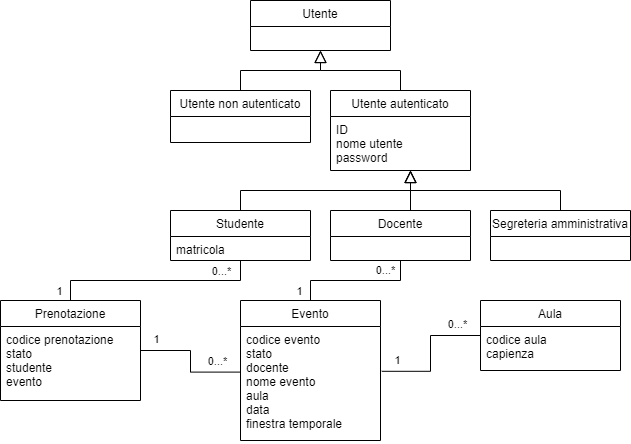
\includegraphics[width=1\textwidth]{Diagramma classi entity.png}
\caption{Diagramma classi entity}
\end{figure}

\subsection{Stereotipi entity/boundary/control}
\begin{figure}[H]
\centering
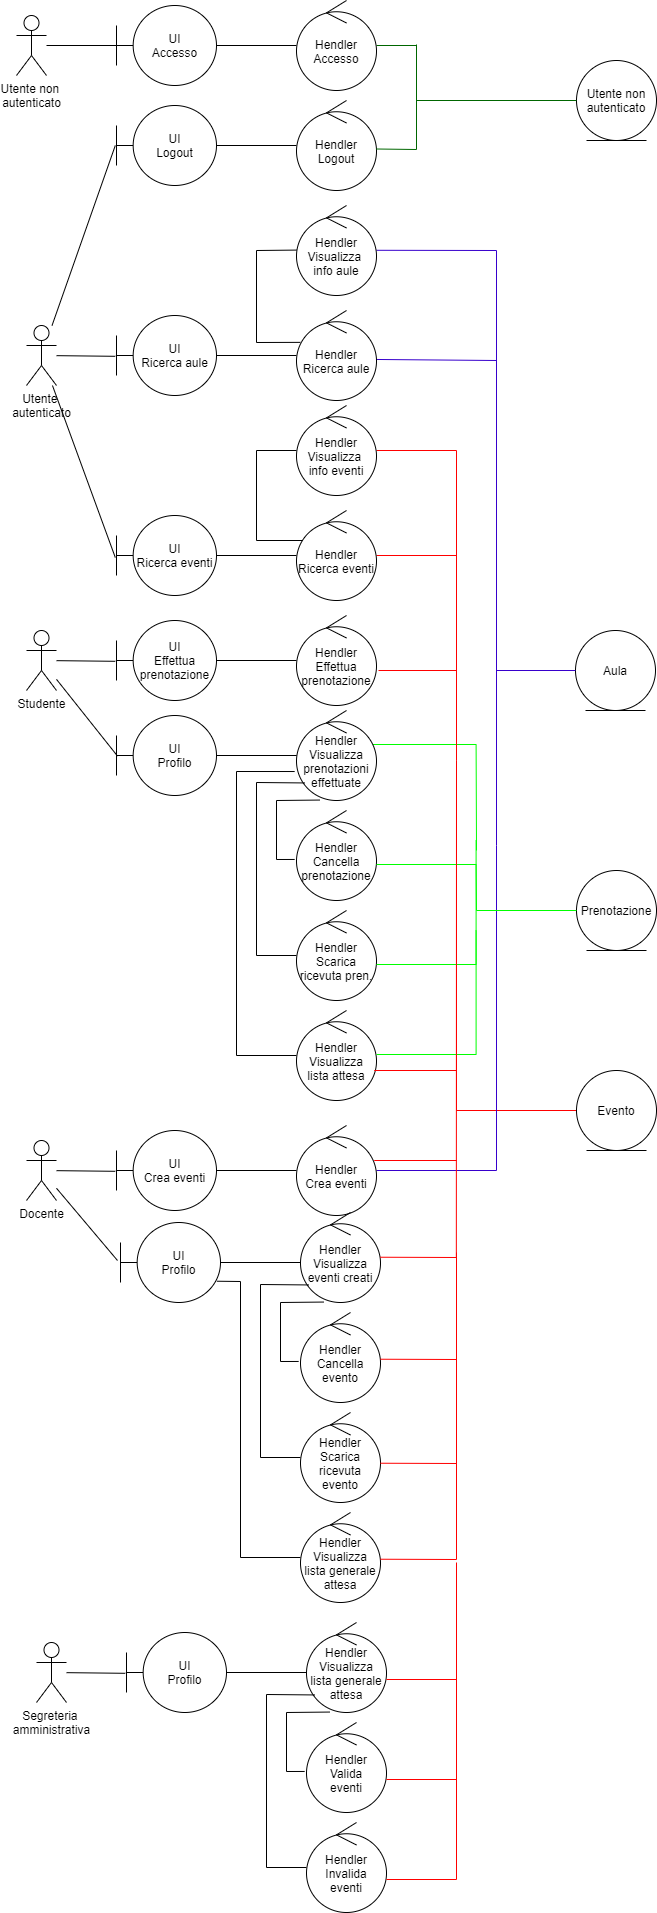
\includegraphics[width=0.42\textwidth]{Diagramma EBC.png}
\caption{Diagramma EBC}
\end{figure}

\subsection{Organizzazione in package}
\begin{figure}[H]
\centering
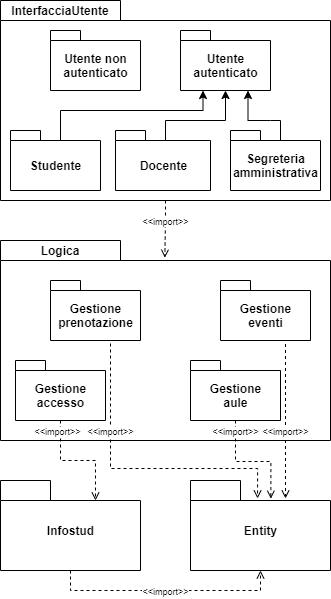
\includegraphics[width=0.72\textwidth]{Organizzazione in package.png}
\caption{Organizzazione in package}
\end{figure}


\section{Progetto}

\subsection{Specifica dell’architettura}
Il sistema é una web application che sfutta un'architettura di tipo client-server. In particolare:
\begin{itemize}
\itemsep0em
\item il server é composto da un application server, che contiene la logica dell'applicazione, da un web server, che ascolta le richieste provenienti dalla rete e da un database manager che gestisce l'accesso al database;
\item il client é composto dai terminali degli utenti del sistema, che comunicano con il web server tramite web browser e protocollo HTTPS.
\end{itemize}
L'application server, inoltre, comunica tramite HTTPS e TCP/IP con il sistema esterno Infostud.\\
Il database sarà unico, dotato di un sistema di failover e di un supporto di archiviazione per il backup.\\
Il sistema sarà protetto da un firewall, che risiederà su un server apposito, e che controllerà e filtrerà le richieste dei client, per garantire maggiore sicurezza al sistema. Per sostenere i picchi e permettere la scalabilità del sistema, il sistema sarà in esecuzione su quattro server in modo ridondante. Il firewall eseguirà un load balancing iniziale per suddividere le richieste tra i due web server presenti, anch'essi ridondanti. A loro volta i due web server effettueranno un load balancing sui server a loro connessi. In questo modo il sistema potrà garantire alta affidabilità anche in caso di fail da parte di uno o più server. Inoltre l'aggiornamento e la manutenzione potranno essere effettuate senza dover spegnere il sistema, eseguendole prima su due server e successivamente sui rimanenti due.

\subsection{Classi di progetto, sottosistemi, componenti}
\begin{figure}[H]
\centering
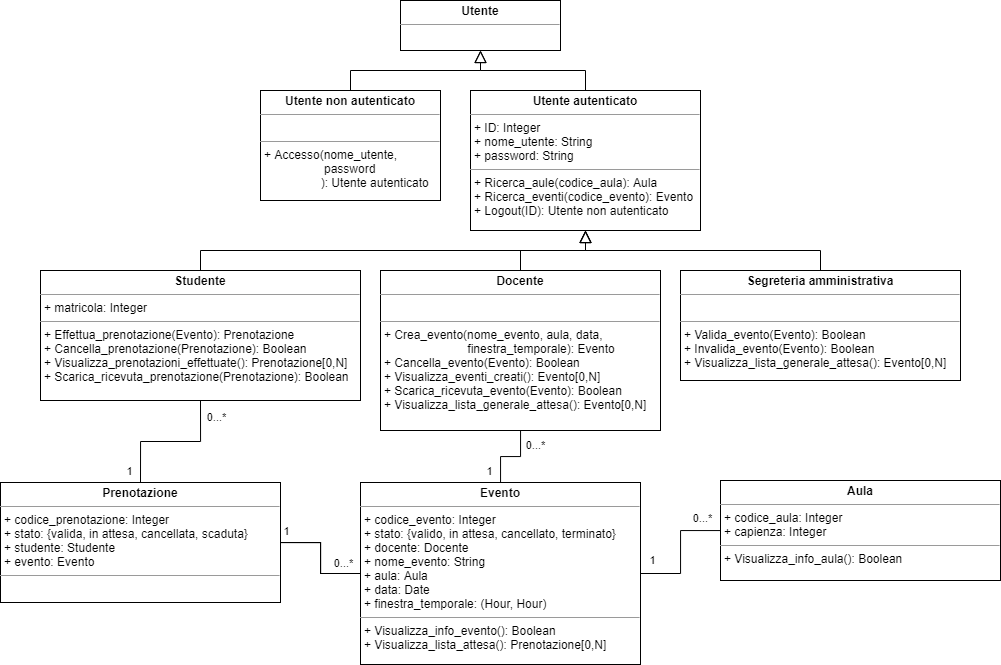
\includegraphics[width=1\textwidth]{Classi di progetto.png}
\caption{Classi di progetto}
\end{figure}

\begin{figure}[H]
\centering
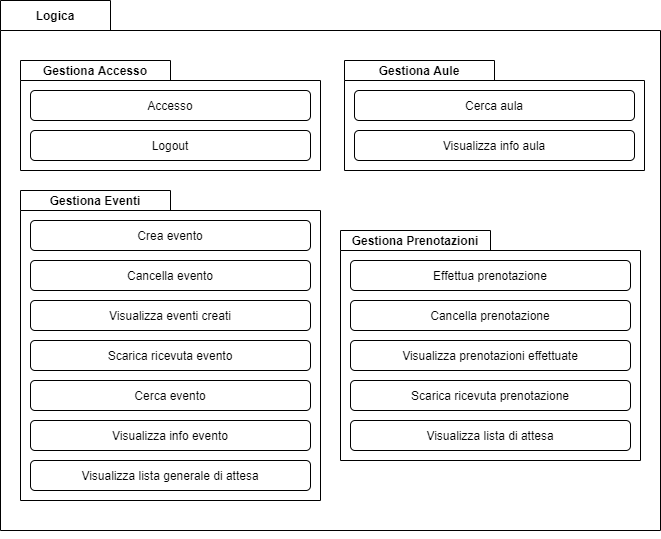
\includegraphics[width=1\textwidth]{Sottosistemi e componenti.png}
\caption{Sottosistemi e componenti}
\end{figure}

\subsection{Realizzazione dei casi d’uso (sequence diagrams)}
\begin{figure}[H]
\centering
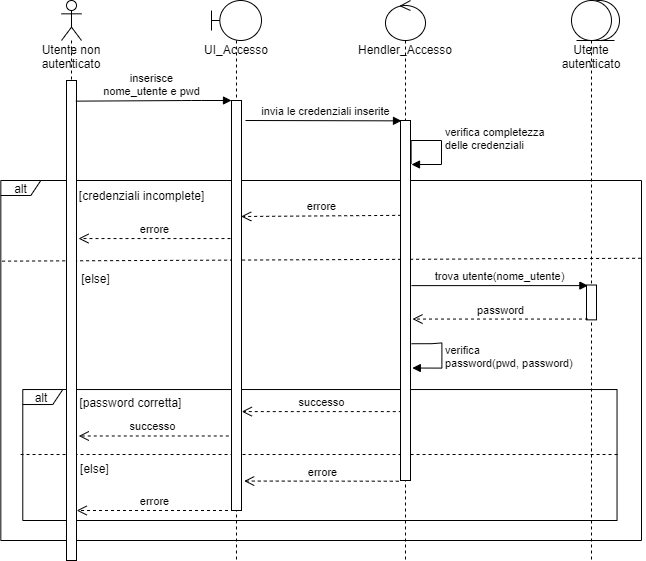
\includegraphics[width=1\textwidth]{SD Gestione accesso - Accesso.png}
\caption{SD Gestione accesso - Accesso}
\end{figure}

\begin{figure}[H]
\centering
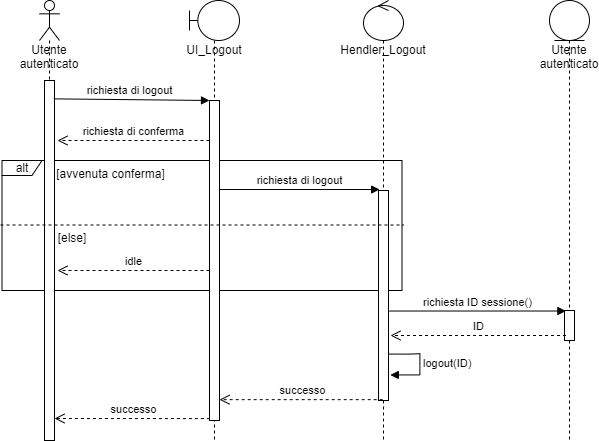
\includegraphics[width=1\textwidth]{SD Gestione accesso - Logout.png}
\caption{SD Gestione accesso - Logout}
\end{figure}

\begin{figure}[H]
\centering
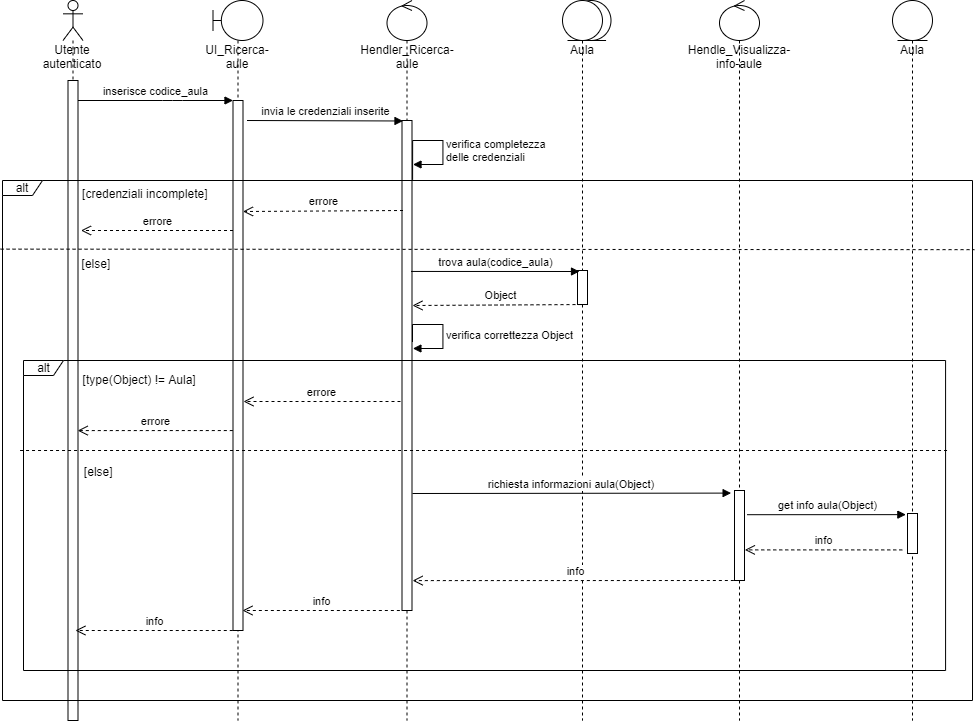
\includegraphics[width=1\textwidth]{SD Gestione aule - Ricerca aule, Visualizza info aule.png}
\caption{SD Gestione aule - Ricerca aule, Visualizza info aule}
\end{figure}

\begin{figure}[H]
\centering
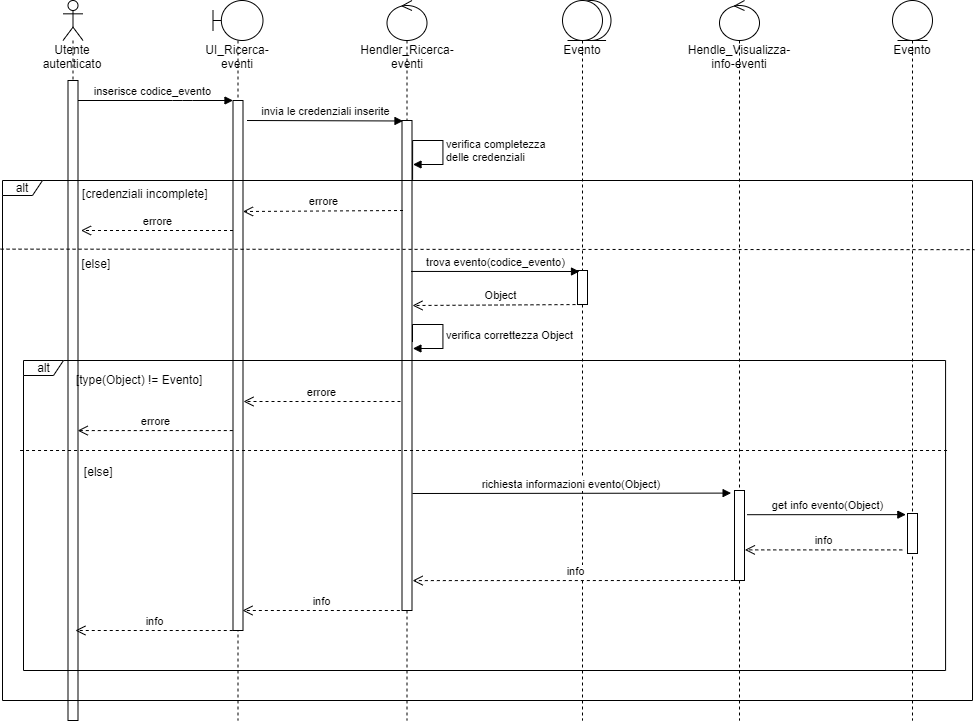
\includegraphics[width=1\textwidth]{SD Gestione eventi - Ricerca eventi, Visualizza info eventi.png}
\caption{SD Gestione eventi - Ricerca eventi, Visualizza info eventi}
\end{figure}

\begin{figure}[H]
\centering
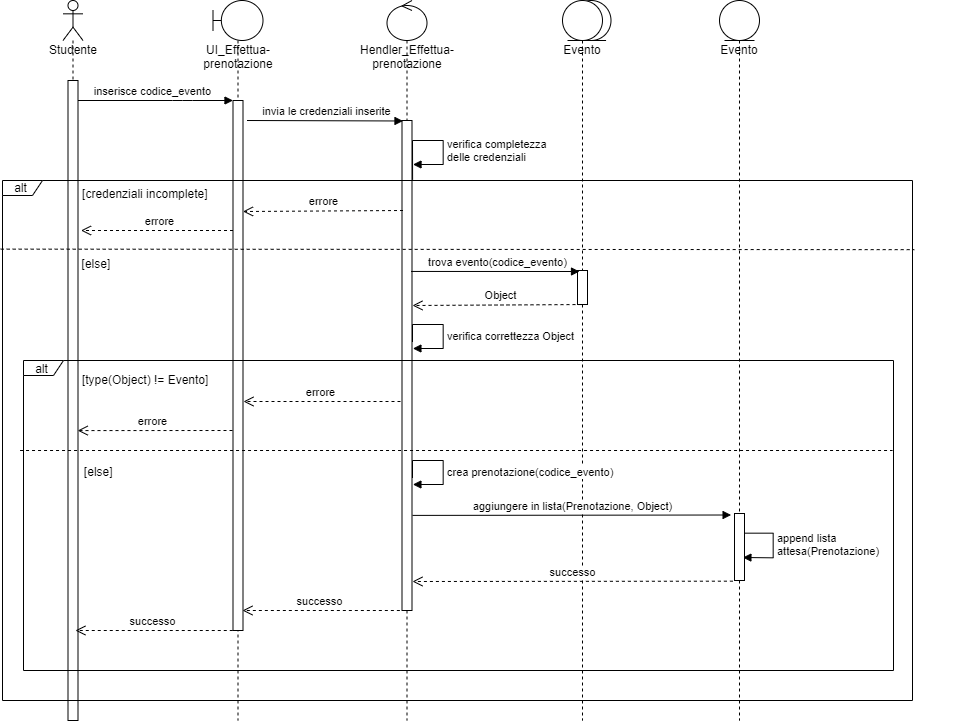
\includegraphics[width=1\textwidth]{SD Gestione prenotazioni - Effettua prenotazione.png}
\caption{SD Gestione prenotazioni - Effettua prenotazione}
\end{figure}

\begin{figure}[H]
\centering
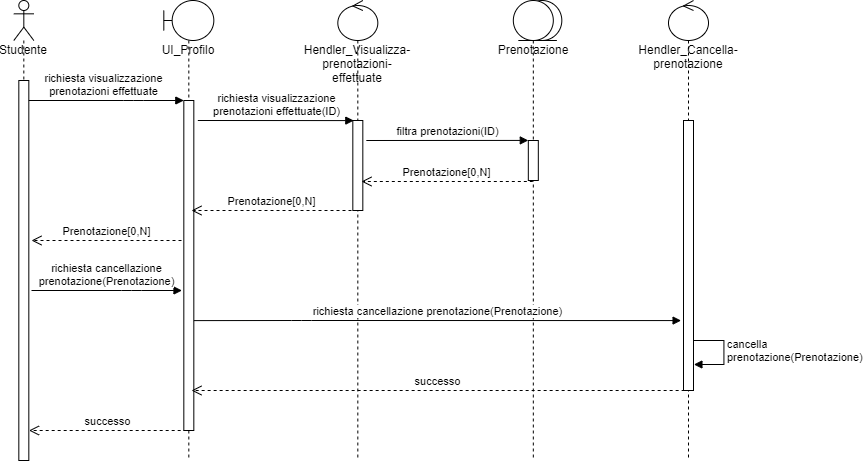
\includegraphics[width=1\textwidth]{SD Gestione prenotazioni - Cancella prenotazione.png}
\caption{SD Gestione prenotazioni - Visualizza prenotazioni effettuate, Cancella prenotazione}
\end{figure}

\begin{figure}[H]
\centering
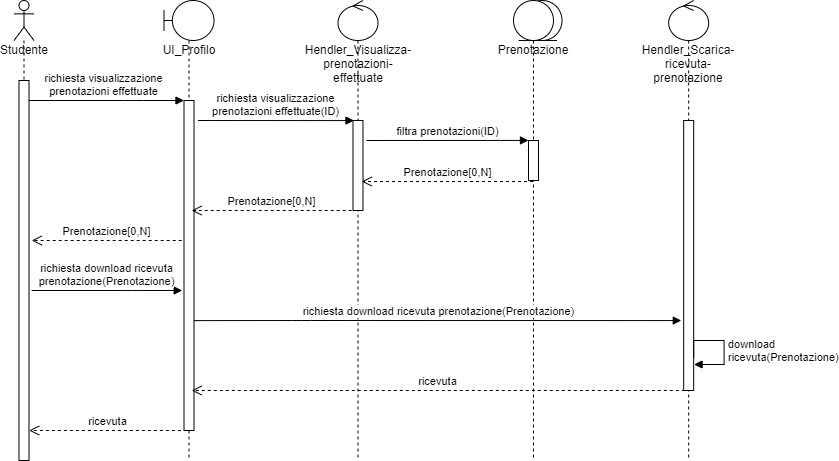
\includegraphics[width=1\textwidth]{SD Gestione prenotazioni - Scarica ricevuta prenotazione.png}
\caption{SD Gestione prenotazioni - Visualizza prenotazioni effettuate, Scarica ricevuta prenotazione}
\end{figure}

\begin{figure}[H]
\centering
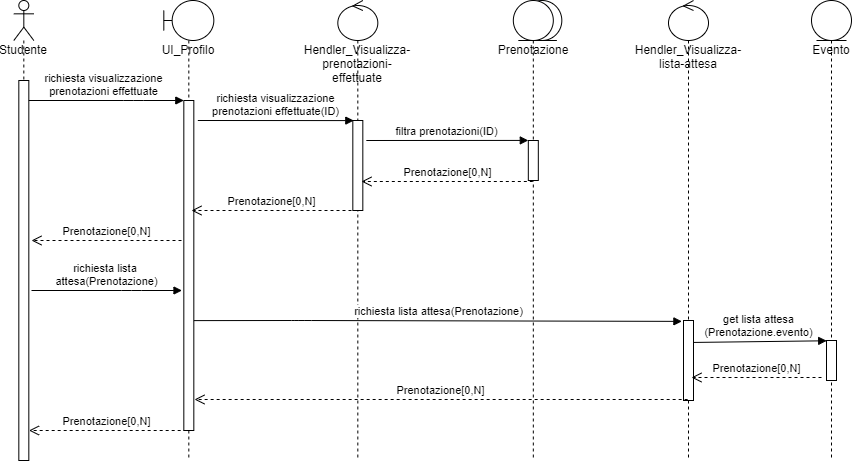
\includegraphics[width=1\textwidth]{SD Gestione prenotazioni - Visualizza lista attesa.png}
\caption{SD Gestione prenotazioni - Visualizza prenotazioni effettuate, Visualizza lista attesa}
\end{figure}

\begin{figure}[H]
\centering
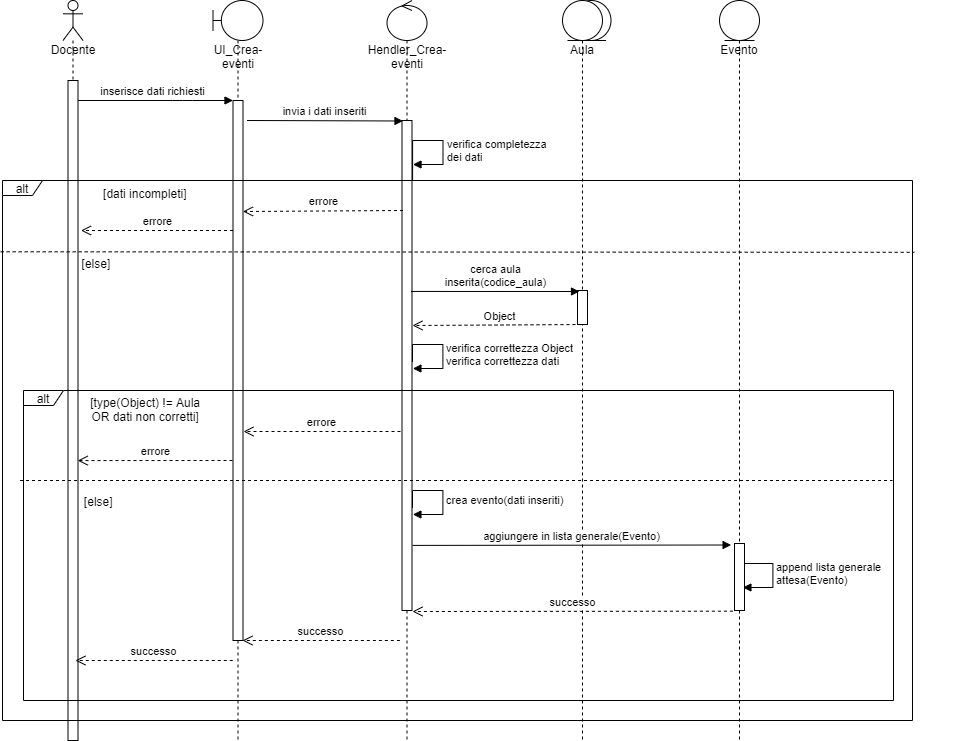
\includegraphics[width=1\textwidth]{SD Gestione eventi - Crea evento.png}
\caption{SD Gestione eventi - Crea eventi}
\end{figure}

\begin{figure}[H]
\centering
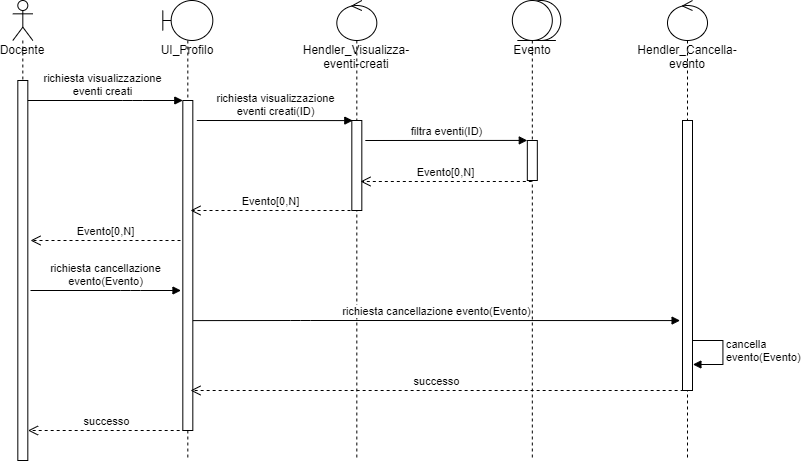
\includegraphics[width=1\textwidth]{SD Gestione eventi - Cancella evento.png}
\caption{SD Gestione eventi - Visualizza eventi creati, Cancella evento}
\end{figure}

\begin{figure}[H]
\centering
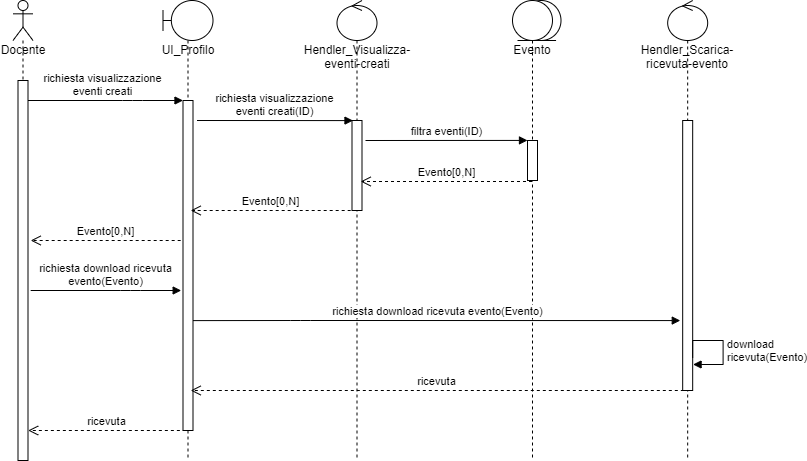
\includegraphics[width=1\textwidth]{SD Gestione eventi - Scarica ricevuta evento creato.png}
\caption{SD Gestione eventi - Visualizza eventi creati, Scarica ricevuta evento}
\end{figure}

\begin{figure}[H]
\centering
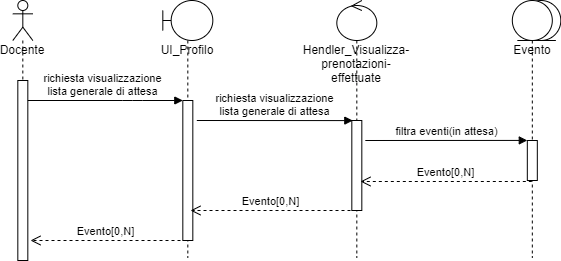
\includegraphics[width=1\textwidth]{SD Gestione eventi - Visualizza lista generale di attesa.png}
\caption{SD Gestione eventi - Visualizza lista generale di attesa}
\end{figure}

\begin{figure}[H]
\centering
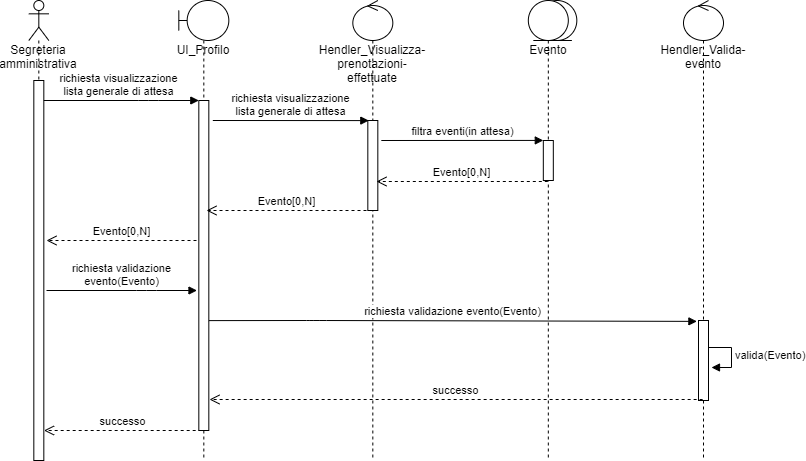
\includegraphics[width=1\textwidth]{SD Gestione eventi - Visualizza lista generale di attesa, Valida evento.png}
\caption{SD Gestione eventi - Visualizza lista generale di attesa, Valida eventi}
\end{figure}

\begin{figure}[H]
\centering
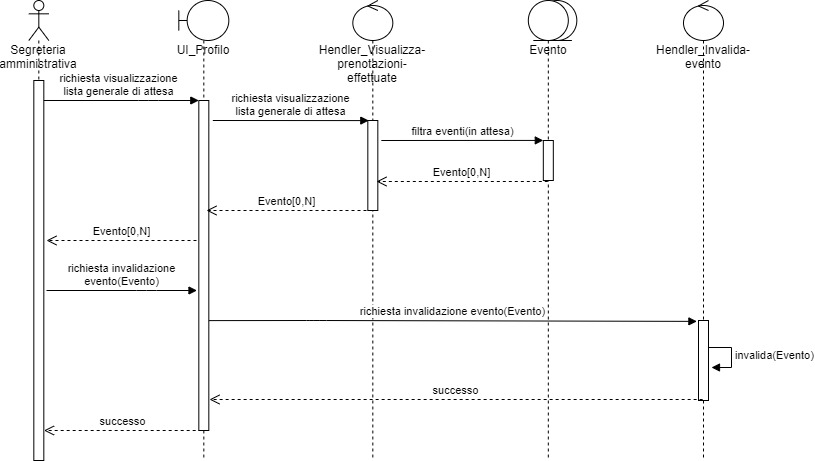
\includegraphics[width=1\textwidth]{SD Gestione eventi - Visualizza lista generale di attesa, Invalida evento.png}
\caption{SD Gestione eventi - Visualizza lista generale di attesa, Invalida eventi}
\end{figure}






\subsection{Cicli di vita di classi significative}
\begin{figure}[H]
\centering
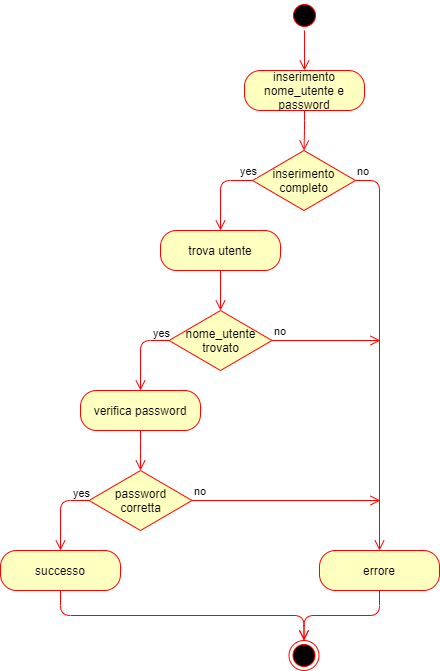
\includegraphics[width=0.8\textwidth]{Ciclo di vita Accesso.png}
\caption{Cico di vita Accesso}
\end{figure}

\begin{figure}[H]
\centering
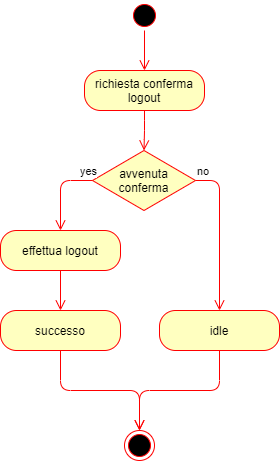
\includegraphics[width=0.55\textwidth]{Ciclo di vita Logout.png}
\caption{Cico di vita Logout}
\end{figure}

\begin{figure}[H]
\centering
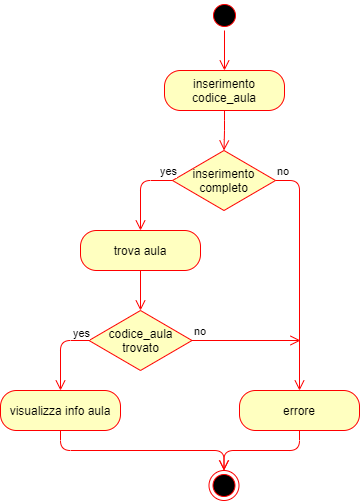
\includegraphics[width=0.65\textwidth]{Ciclo di vita Ricerca aule, Visualizza info.png}
\caption{Ciclo di vita Ricerca aule, Visualizza info aule}
\end{figure}

\begin{figure}[H]
\centering
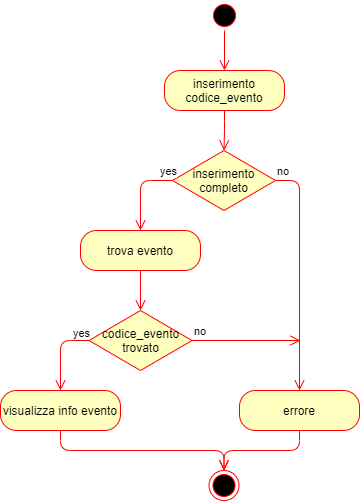
\includegraphics[width=0.65\textwidth]{Ciclo di vita Ricerca eventi, Visualizza info.png}
\caption{Ciclo di vita Ricerca eventi, Visualizza info eventi}
\end{figure}

\begin{figure}[H]
\centering
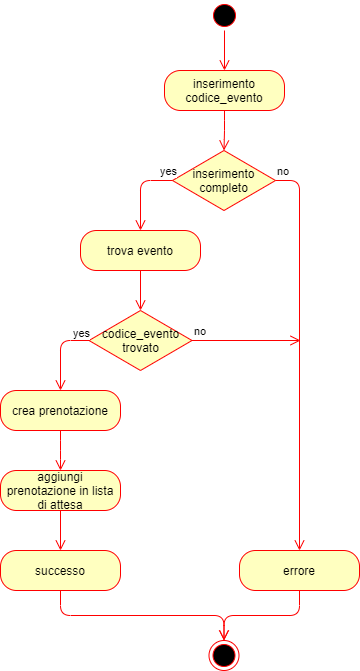
\includegraphics[width=0.65\textwidth]{Ciclo di vita Effettua prenotazione.png}
\caption{Ciclo di vita Effettua prenotazione}
\end{figure}

\begin{figure}[H]
\centering
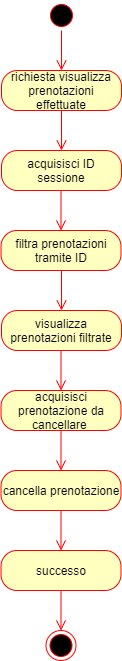
\includegraphics[width=0.225\textwidth]{Ciclo di vita Visualizza prenotazioni, Cancella prenotazione.png}
\caption{Ciclo di vita Visualizza prenotazioni effettuate, Cancella prenotazione}
\end{figure}

\begin{figure}[H]
\centering
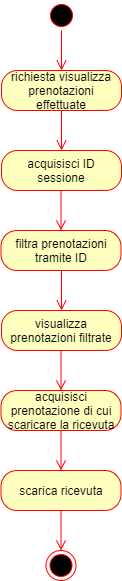
\includegraphics[width=0.225\textwidth]{Ciclo di vita Visualizza prenotazioni, Scarica ricevuta prenotazione.png}
\caption{Ciclo di vita Visualizza prenotazioni effettuate, Scarica ricevuta prenotazione}
\end{figure}

\begin{figure}[H]
\centering
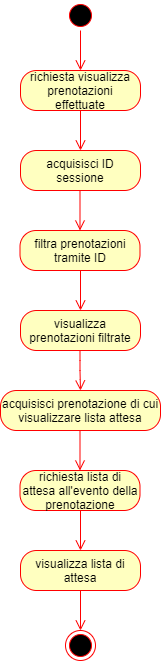
\includegraphics[width=0.3\textwidth]{Ciclo di vita Visualizza prenotazioni, Visualizza lista attesa.png}
\caption{Ciclo di vita Visualizza prenotazioni effettuate, Visualizza lista di attesa}
\end{figure}

\begin{figure}[H]
\centering
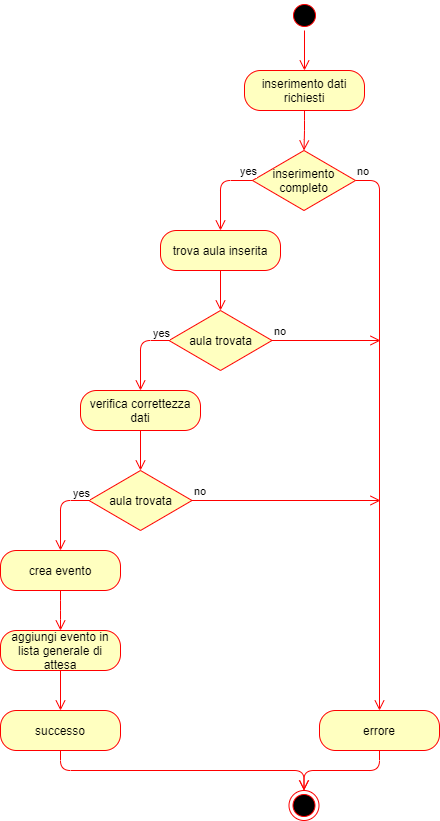
\includegraphics[width=0.7\textwidth]{Ciclo di vita Crea evento.png}
\caption{Ciclo di vita Crea evento}
\end{figure}

\begin{figure}[H]
\centering
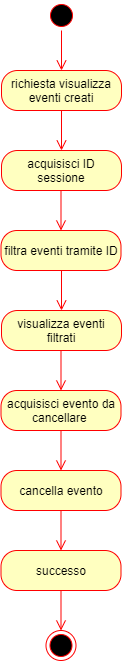
\includegraphics[width=0.225\textwidth]{Ciclo di vita Visualizza eventi creati, Cancella evento.png}
\caption{Ciclo di vita Visualizza eventi creati, Cancella evento}
\end{figure}

\begin{figure}[H]
\centering
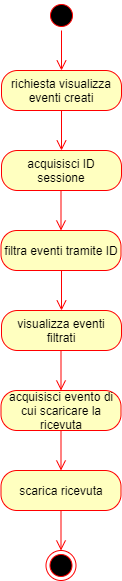
\includegraphics[width=0.225\textwidth]{Ciclo di vita Visualizza eventi creati, Scarica ricevuta evento.png}
\caption{Ciclo di vita Visualizza eventi creati, Scarica ricevuta evento}
\end{figure}

\begin{figure}[H]
\centering
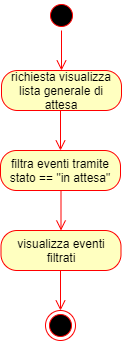
\includegraphics[width=0.25\textwidth]{Ciclo di vita Visualizza lista generale di attesa.png}
\caption{Ciclo di vita Visualizza lista generale di attesa}
\end{figure}

\begin{figure}[H]
\centering
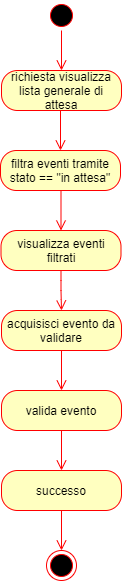
\includegraphics[width=0.225\textwidth]{Ciclo di vita Visualizza lista generale di attesa, Valida eventi.png}
\caption{Ciclo di vita Visualizza lista generale di attesa, Valida eventi}
\end{figure}

\begin{figure}[H]
\centering
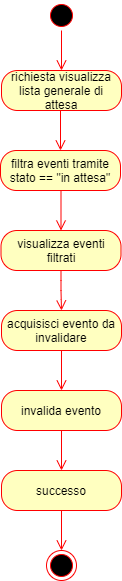
\includegraphics[width=0.225\textwidth]{Ciclo di vita Visualizza lista generale di attesa, Invalida eventi.png}
\caption{Ciclo di vita Visualizza lista generale di attesa, Invalida eventi}
\end{figure}

\end{document}

